\documentclass[12pt]{article}

\usepackage{hcmus-report-template}

% Disable indentation on new paragraphs
\setlength{\parindent}{0pt}

% Line spacing 1.5
\renewcommand{\baselinestretch}{1.5}

% Optional: graphic path
% \graphicspath{PATH_TO_GRAPHIC_FOLDER}

% To use Times font family, uncomment this row
% \usepackage{mathptmx}

% To use roman section / subsection, uncomment these rows
% \renewcommand{\thesection}{\Roman{section}}
% \renewcommand{\thesubsection}{\thesection.\Roman{subsection}}

% Define course name, report name and report title.
\newcommand{\coursename}{CS420}
\newcommand{\reportname}{Ares’s adventure}
\newcommand{\reporttitle}{Project 1. Search}

\newcommand{\studentname}{Le Van Cuong - 22125013\\22125079 - Nguyễn Minh Quân\\Bui Danh Nghe - 22125063\\Phung Khanh Vinh - 22125122}


% Header
\lhead{\reporttitle}
\rhead{
%Trường Đại học Khoa học Tự nhiên - ĐHQG HCM
\\
\coursename
}

% Footer
%\newcommand{\leftfooter}{\LaTeX\ by \href{https://github.com/trhgquan}{Quan, Tran Hoang}}
%\lfoot{\leftfooter}

% ============ DOCUMENT ============
\begin{document}

\pagenumbering{roman}
\begin{titlepage}
\newcommand{\HRule}{\rule{\linewidth}{0.5mm}}
\centering

\textsc{\LARGE}\\[0.5cm]
\textsc{\Large }\\[0.5cm]
\textsc{\large}\\[0.5cm]
\textsc{}\\[0.5cm]

\HRule \\[0.4cm]
{ 
\huge{\bfseries{\reporttitle}}\\[0.5cm]
\large{\bfseries{\reportname}}
}\\[0.4cm]
\HRule \\[0.5cm]

\textbf{\large \coursename}\\[0.5cm]

\begin{minipage}[t]{0.4\textwidth}
\begin{flushleft} \large
\emph{Group's member:}\\
\studentname
\end{flushleft}
\end{minipage}\\[1cm]
~
%
%\begin{minipage}[t]{0.4\textwidth}
%\begin{flushright} \large
%\emph{Giáo viên hướng dẫn:} \\
%\teachername
%\end{flushright}
%\end{minipage}\\[1cm]
%

%
\includegraphics[scale=.20]{img/hcmus-logo.png}\\[1cm] 

\vfill
\end{titlepage}
	

\tableofcontents
\pagebreak
\listoftables
\pagebreak
\listoffigures
\pagebreak

\pagenumbering{arabic}
\setcounter{page}{1}

\section{Task Distribution}

\begin{table}[H]
\captionof{table}{Task Distribution}
\hline
\begin{tabular}{l|llll}
\\
                                        &  (22125013) & (22125015) & (22125063) & (22125122) \\
                                        \hline
Dataset Finding (10\% Total)            & \textbf{}               &                            & 5\%                      & 5\%                         \\
Model Building (40\% Total)             & 10\%                    & 20\%                       & 5\%                      & 5\%                         \\
Report Writing \& Research (40\% Total) & 15\%                    &                            & 15\%                     & 10\%                        \\
Validation + Proof Reading (10\% Total) & \textbf{}               & 5\%                        &                          & 5\%                         \\
\hline
Total                                   & 25\%                    & 25\%   
& 25\%                     & 25\%                       
\end{tabular}
\end{table}
\section{Self-evaluation}



\section{Algorithm Explaination}
%\section{Section}

\subsection{Một số lưu ý}

\subsubsection{Cài đặt offline}
Template này yêu cầu cài đặt một số gói (package) nâng cao cho TexStudio:
\begin{itemize}
\item Để gõ thuật toán: \texttt{algorithm} và \texttt{algpseudocode}
\item Để nhúng (chèn) code: \texttt{listings}
\end{itemize}
Các gói này được cài đặt thông qua lệnh
\begin{lstlisting}[language=sh]
sudo apt-get install texlive-full
\end{lstlisting}
Tuy nhiên kích thước gói đâu đó vào khoảng 5GB (!). Vì vậy tốt nhất nên xài Overleaf.

\subsubsection{Sử dụng font khác}
Tham khảo font typefaces tại \href{https://www.overleaf.com/learn/latex/Font_typefaces}{link này}.

\subsubsection{Đánh số chỉ mục bằng chữ số La Mã}
Mở file \texttt{main.tex} và bỏ comment dòng 
\begin{lstlisting}[language=tex]
% \renewcommand{\thesection}{\Roman{section}}
% \renewcommand{\thesubsection}{\thesection.\Roman{subsection}}  
\end{lstlisting}

\subsection{Ví dụ}
Ngày xửa ngày xưa, ở vương quốc VNUHCM - US, có một chàng hoàng tử ngồi cắm đầu viết doc\footnote{Đây là footnote, chú thích lại những gì cần chú ý.}.\\
Mặc định muốn xuống dòng chỉ cần dùng $\backslash\backslash$  (2 lần dấu xẹt huyền).\\
Nếu bạn muốn thụt đầu dòng khi bắt đầu paragraph mới, vào \texttt{main.tex} và disble dòng
\begin{lstlisting}[language=tex]
\setlength{\parindent}{0pt}
\end{lstlisting}

\subsection{First subsection}
\subsubsection{First sub-subsection}
Subsection để ví dụ thôi. Thêm vài ví dụ:
\begin{itemize}
    \item Dùng itemize
    \item Vẫn là itemize
\end{itemize}
Sau đó xài enumerate:
\begin{enumerate}
    \item Dùng enumerate
    \item Vẫn là enumerate
\end{enumerate}
Nhỏ hơn subsubsection thì xài \texttt{paragraph}:

\paragraph{Đây là ví dụ cho paragraph}
Lưu ý là paragraph không nằm trong Mục lục.

\subsection{Chia nhỏ nội dung}
Bạn có thể chia nhỏ nội dung của báo cáo thành các file \texttt{.tex} và dùng lệnh \texttt{input} để chèn vào báo cáo chính. Ví dụ có trong file \texttt{main.tex}.

%\newpage
\section{Question 2 - Dataset 1}
\subsection{Introduction}
This report analyzes a dataset containing various features related to restaurants and their revenue. The goal is to explore relationships between different variables and the revenue, and to generate insights that may help in predicting future revenue for restaurants.

\subsection{Dataset Overview}
The dataset contains 8,368 records of restaurants with the following key features:
\begin{itemize}
    \item \textbf{Name}: Name of the restaurant.
    \item \textbf{Location}: The location of the restaurant (Downtown, Rural, Suburban).
    \item \textbf{Cuisine}: The type of cuisine offered by the restaurant (e.g., American, Italian, Japanese).
    \item \textbf{Rating}: Average rating of the restaurant (scale of 1 to 5).
    \item \textbf{Seating Capacity}: The number of seats available at the restaurant.
    \item \textbf{Average Meal Price}: The average price of a meal.
    \item \textbf{Marketing Budget}: The marketing budget of the restaurant.
    \item \textbf{Social Media Followers}: Number of social media followers.
    \item \textbf{Chef Experience}: The number of years of experience the chef has.
    \item \textbf{Number of Reviews}: Total number of reviews received.
    \item \textbf{Average Review Length}: The average length of the reviews.
    \item \textbf{Ambience Score}: Score reflecting the ambience of the restaurant (scale of 1 to 10).
    \item \textbf{Service Quality Score}: Score reflecting the quality of service (scale of 1 to 10).
    \item \textbf{Parking Availability}: Whether parking is available (Yes/No).
    \item \textbf{Weekend Reservations}: Number of reservations during weekends.
    \item \textbf{Weekday Reservations}: Number of reservations during weekdays.
    \item \textbf{Revenue}: The total revenue generated by the restaurant.
\end{itemize}
\subsubsection{Data Cleaning}
The dataset had no missing values, so the main focus was on transforming categorical variables like \textit{Location}, \textit{Cuisine}, and \textit{Parking Availability} into factors for analysis. Imputations for missing values would involve replacing them with median values if necessary.

\subsubsection{Descriptive Statistics}
Table \ref{tab:descriptive} provides a summary of key statistics for the numeric variables in the dataset.

\begin{table}[H]
\centering
\caption{Descriptive Statistics of the Dataset}
\label{tab:descriptive}
\begin{tabular}{lrrrrr}
\toprule
Variable & Mean & Median & Min & Max & SD \\
\midrule
Revenue (in \$) & 656,070 & 604,242 & 184,709 & 1,531,868 & 267,414 \\
Rating & 4.01 & 4.00 & 3.00 & 5.00 & 0.50 \\
SeatingCapacity & 60.21 & 60.00 & 30.00 & 90.00 & 16.57 \\
AverageMealPrice (in \$) & 47.90 & 45.53 & 25.00 & 76.00 & 13.86 \\
MarketingBudget (in \$) & 3,218 & 2,846 & 604 & 9,978 & 1,673 \\
SocialMediaFollowers & 36,191 & 32,519 & 5,277 & 103,777 & 19,830 \\
ChefExperience (Years) & 10.05 & 10.00 & 1 & 19 & 5.47 \\
NumberofReviews & 523 & 528 & 50 & 999 & 275 \\
\bottomrule
\end{tabular}
\end{table}
\newpage
\subsubsection{Data Visualization}
\paragraph{Revenue vs. Average Meal Price}
The relationship between revenue and average meal price is visualized in Figure \ref{fig:revenue_price}. A positive linear trend can be observed, suggesting that restaurants with higher average meal prices tend to generate more revenue.

\begin{figure}[H]
\centering
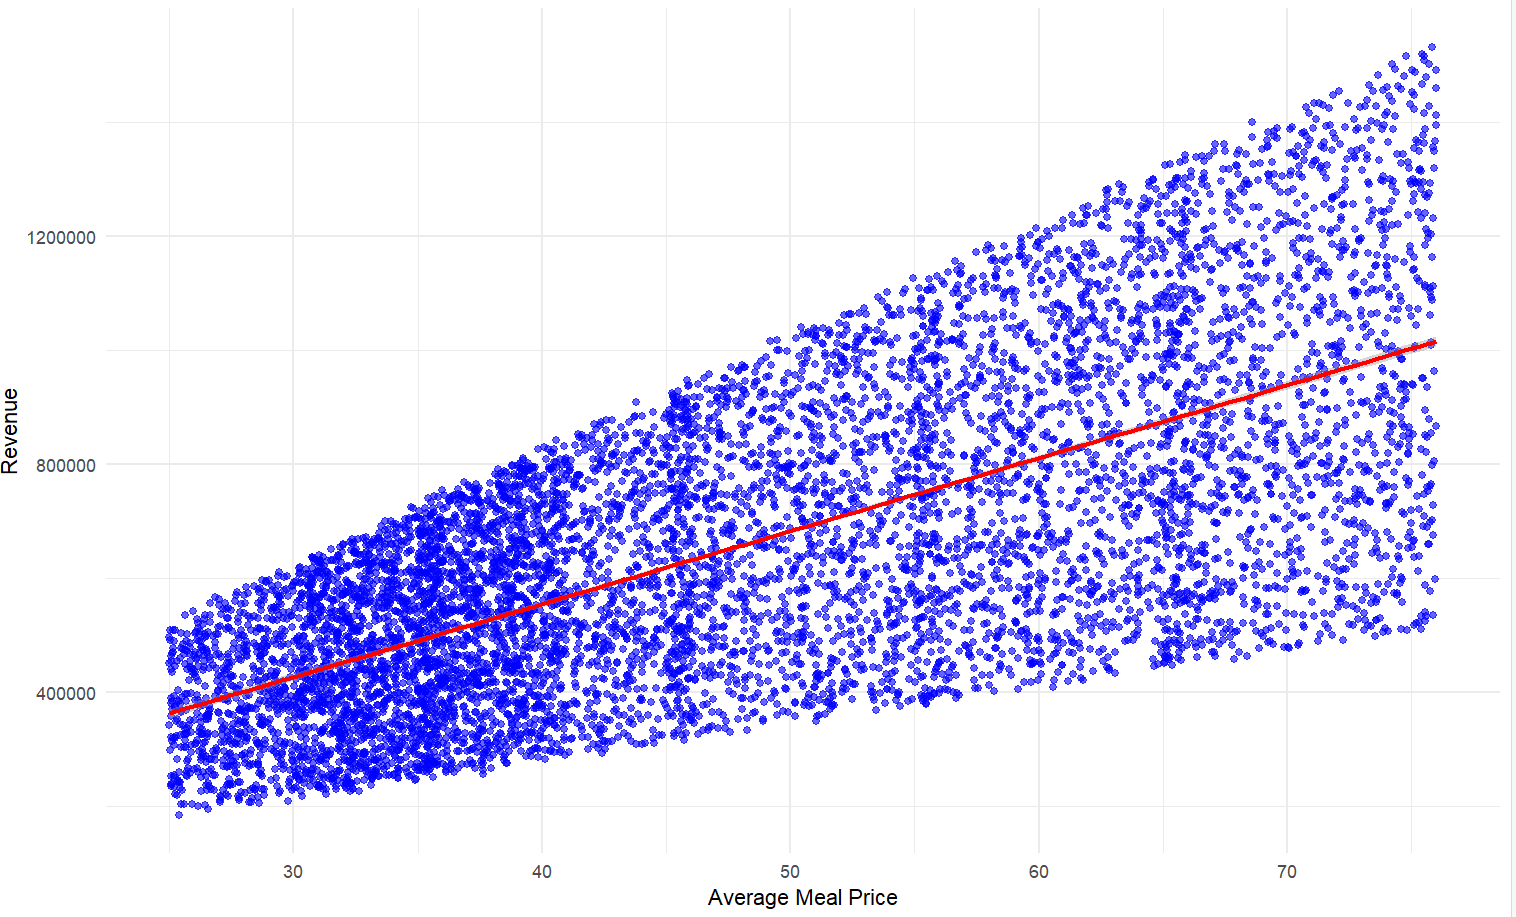
\includegraphics[width=0.7\textwidth]{img/d1.png}
\caption{Scatter Plot: Revenue vs. Average Meal Price}
\label{fig:revenue_price}
\end{figure}

\paragraph{Revenue by Cuisine Type}
Figure \ref{fig:revenue_cuisine} shows the distribution of revenue across different cuisine types. Certain cuisines, such as Japanese and French, tend to have higher median revenues.

\begin{figure}[H]
\centering
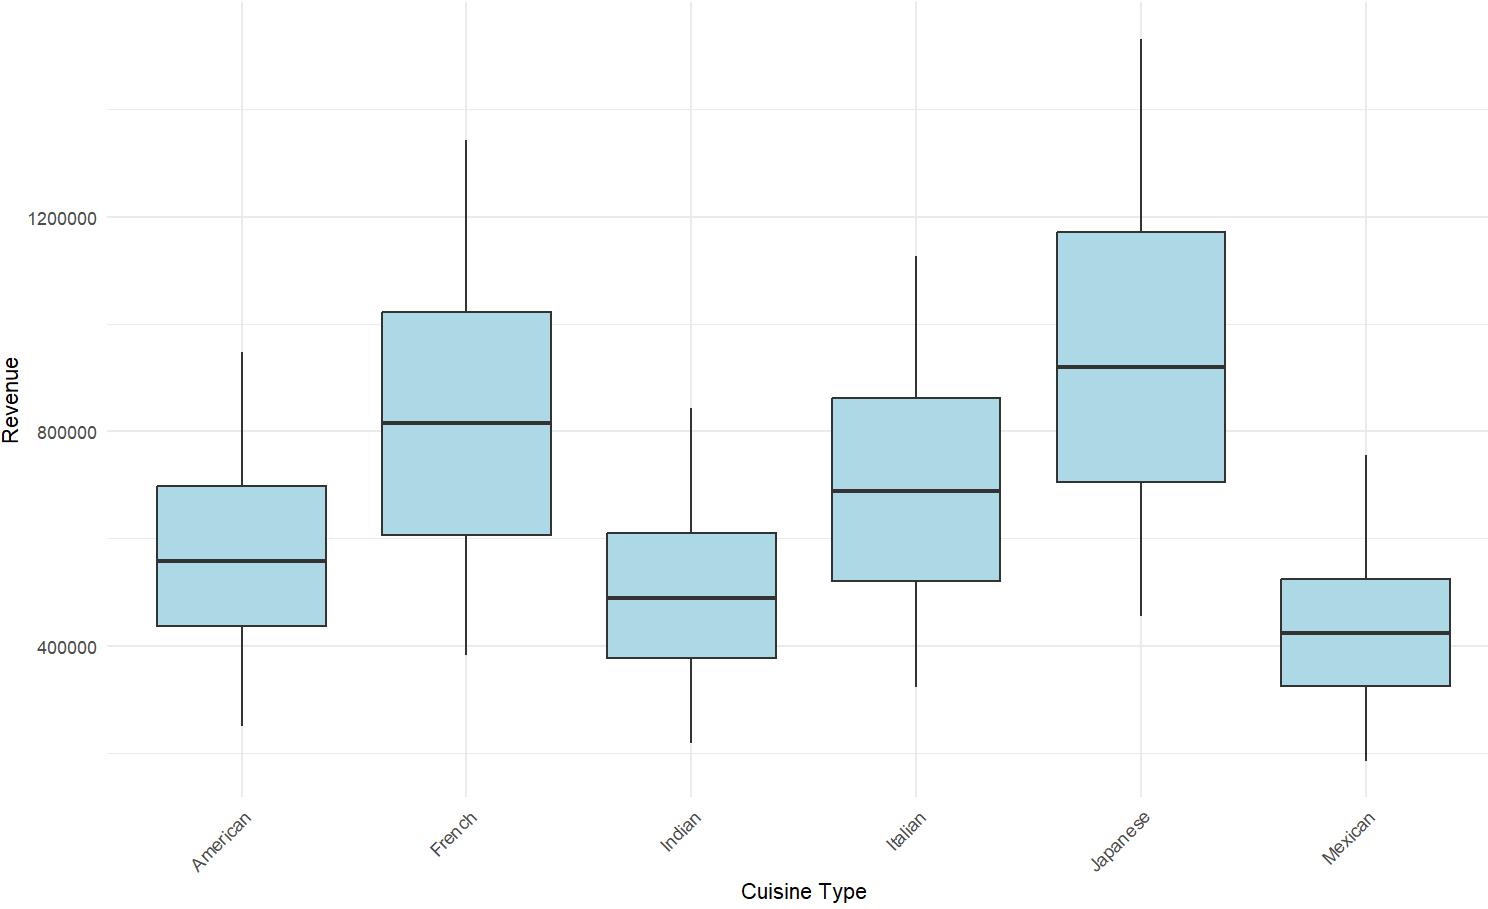
\includegraphics[width=0.7\textwidth]{img/d2.png}
\caption{Boxplot: Revenue by Cuisine Type}
\label{fig:revenue_cuisine}
\end{figure}

\subsubsection{Correlation Analysis}
A correlation analysis was conducted to identify relationships between numeric variables. Figure \ref{fig:correlation} presents a correlation heatmap that highlights strong correlations, such as between seating capacity and revenue, and between average meal price and revenue.

\begin{figure}[H]
\centering
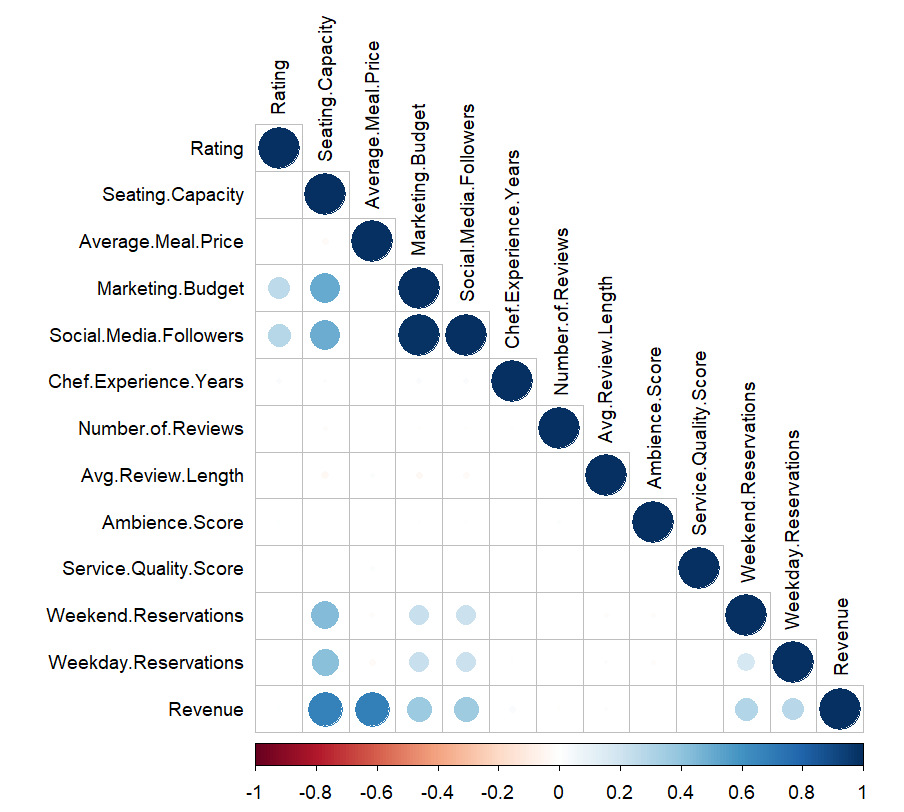
\includegraphics[width=0.7\textwidth]{img/d3.png}
\caption{Correlation Matrix}
\label{fig:correlation}
\end{figure}
\subsubsection{Distribution of Scaled Revenue}
The distribution of scaled revenue (revenue divided by seating capacity) is visualized in Figure \ref{fig:scaled_revenue_distribution}. This metric helps normalize revenue across restaurants of different sizes, providing a more equitable comparison.

\begin{figure}[H]
\centering
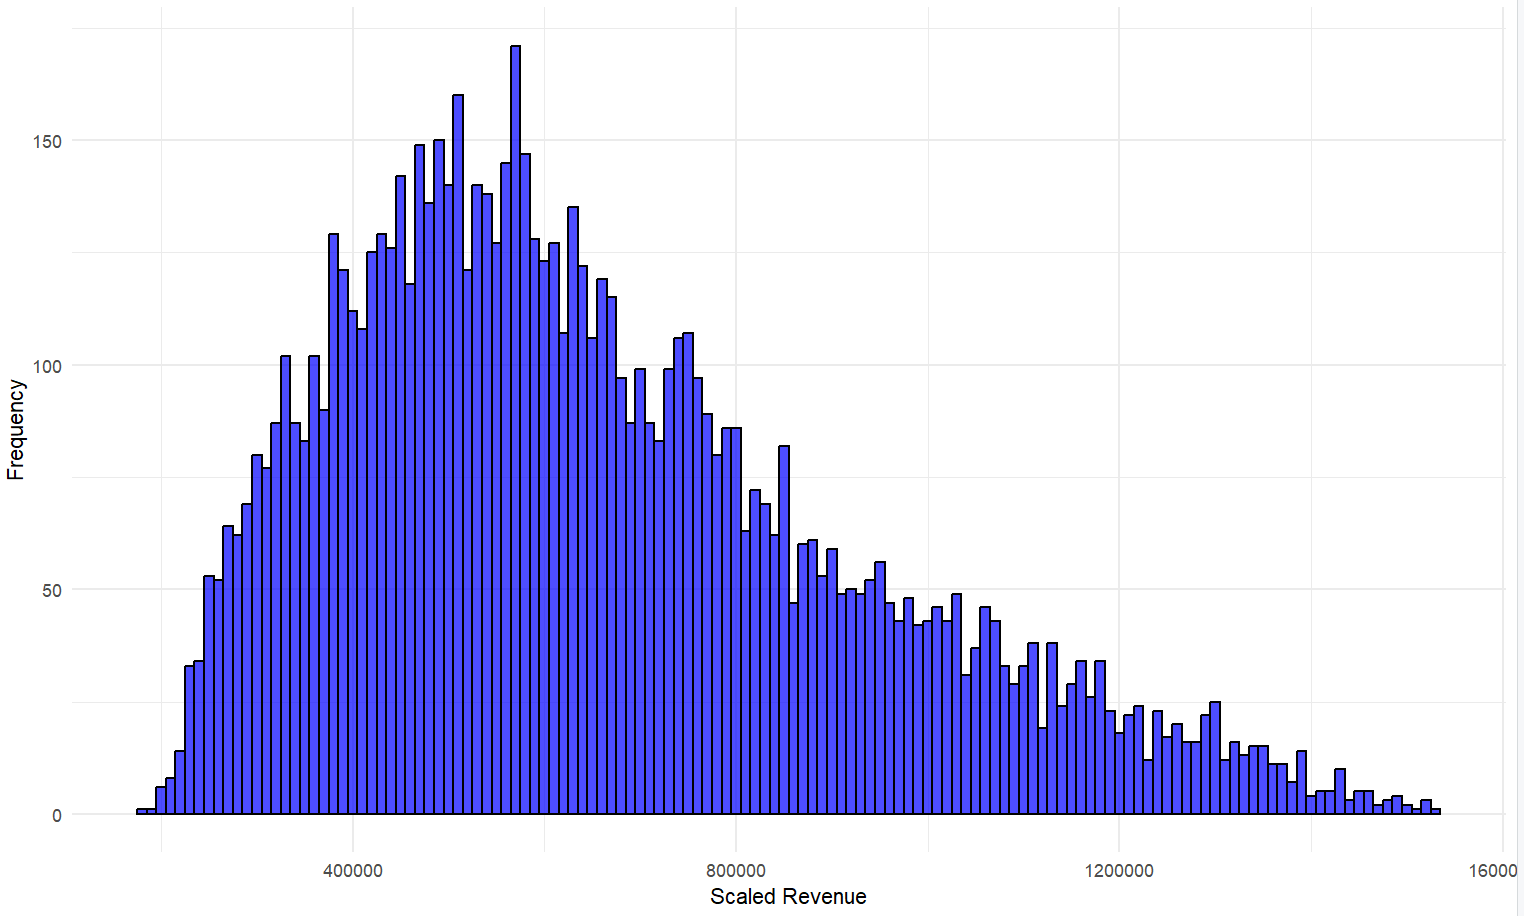
\includegraphics[width=0.7\textwidth]{img/d4.png}
\caption{Histogram: Distribution of Scaled Revenue (Revenue per Seat)}
\label{fig:scaled_revenue_distribution}
\end{figure}

The histogram shows that while most restaurants fall within a certain range of scaled revenue, there are a few outliers with significantly higher or lower revenue per seat. This could be indicative of unique business models or market conditions.

\subsection{Data splitting}

The data is split into two part, training dataset and validation dataset. Training dataset contains 80$\%$ of the observations and the validation dataset contains 80$\%$ of the observations. The split is performed randomly with RStudio.

For replication, we use the seed 777489.

\subsection{Model building}
\subsubsecction{Baseline model}
When inspecting the interaction between indicators, we notice that the interaction term between 'SeatingCapacity' and 'AverageMealPrice' can practically determines 'Revenue' alone, as shown by the plot below:

\begin{figure}[H]
\centering
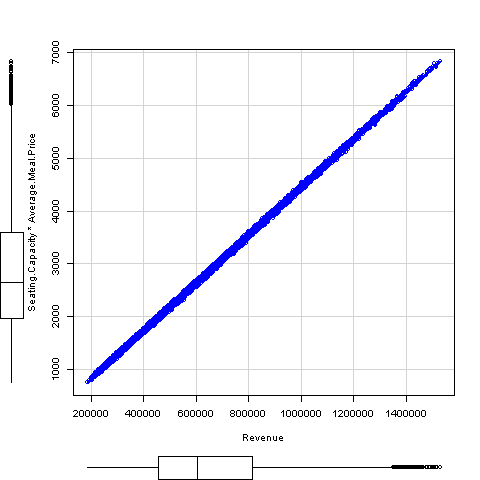
\includegraphics[width=0.7\textwidth]{img/scattertrip.png}
\caption{Scatterplot: Revenue by SeatingCapacity*AverageMealPrice}
\label{fig:scaled_revenue_distribution}
\end{figure}

Thus, we choose the baseline model to be: 
\begin{center}
$
M: \ Revenue \ = \beta_0 + \beta_1 \left(\text{SeatingCapacity} \times(\text{AverageMealPrice})\right)
$
\end{center}

\subsection{Improvement to a new model}

So our baseline model have the form of:

\begin{center}
$
M: \ Revenue \ = \beta_0 + \beta_1 \left(\text{SeatingCapacity} \times(\text{AverageMealPrice})\right)
$
\end{center}

So with such a high $R^2$ and such simple formula for the baseline, it is unneccessary to construct a improved model. In addition, to build a model with $R^2$ and adjust $R^2$ surpassing $99,9\%$ is no simple task. 

Hence, the main aim for our new model is to fix a problem of the baseline model: The error of the baseline model is not normal distributed. As many statistical tests, like t-tests and F-tests, rely on the assumption of normally distributed errors. These tests allow us to draw inferences about population parameters based on sample data. 

Luckily, as our baseline model has high $R^2$ and adjust $R^2$ already, we can sacrifice some accuracy for normalizing the error.

\subsubsection{Addition of indicators}
We start by determine which other variables can indicate the 'Revenue'. From all the indicators available, only 'WeekdayReservation' and 'WeekendReservation' shows signs of indication, but not so much. 
\begin{figure}[H]
\centering
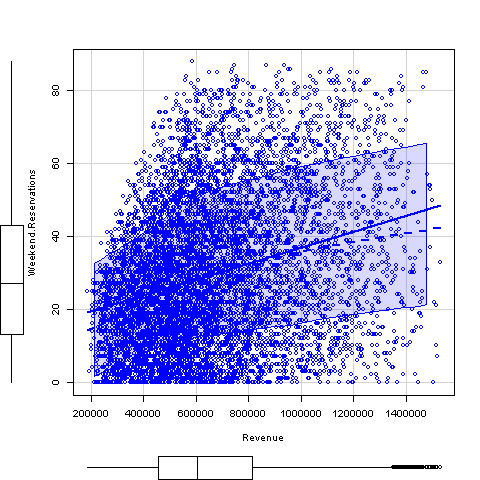
\includegraphics[width=0.7\textwidth]{img/scatterthat.png}
\caption{Scatterplot: Revenue by Reservation}
\label{fig:scaled_revenue_distribution_reservation}
\end{figure}

Drawing the histogram of the two, we also see that while the distribution is fairly normalized, it is skewed. 
\begin{figure}[H]
\centering
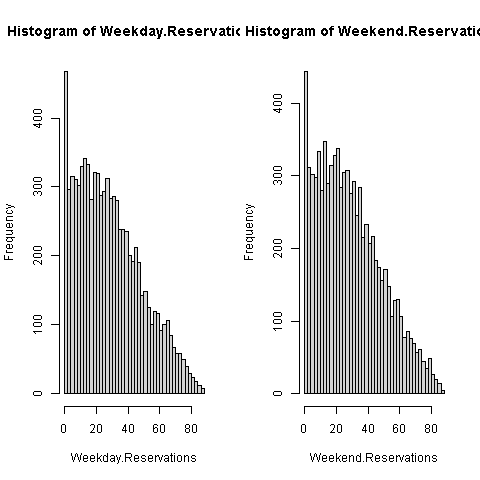
\includegraphics[width=0.7\textwidth]{img/scatterthis.png}
\caption{Histogram of the reservations}
\label{fig:scaled_hist_distribution_reservation}
\end{figure}
Therefore, we perform boxcox transformation on the two of them and indicate the $\lambda$ value to be close to 0.5. As a result, we add the two terms $\sqrt{WeekdayReservation}$ and $\sqrt{WeekdayReservation}$ into the model.

\subsubsection{Interaction terms}
In order to improve the model to ensure the normality of the residuals, we inspect the interaction terms between a quantitative indicator and a qualitative one. After checking all the interaction terms we can, we conclude that the interaction terms that have an impact on the response is SeatingCapacity*Location and AverageMealPrice*Cuisine, as shown by the graphs below:
\begin{figure}[H]
\centering
\begin{subfigure}{.5\textwidth}
  \centering
  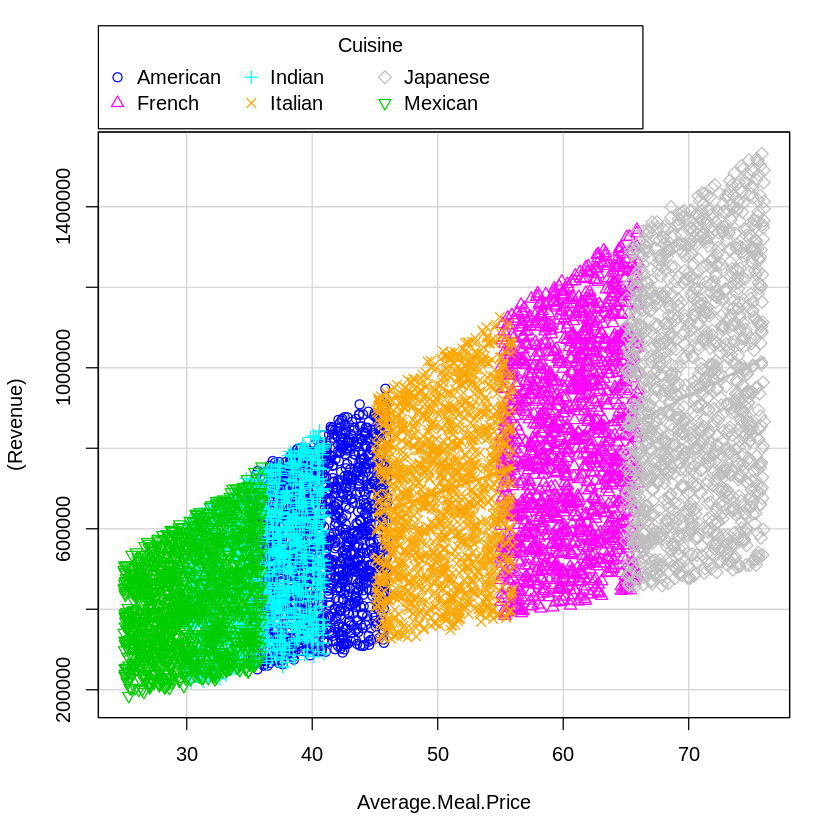
\includegraphics[width=.4\linewidth]{img/revByMealGroupCuisine.png}
\end{subfigure}%
\begin{subfigure}{.5\textwidth}
  \centering
  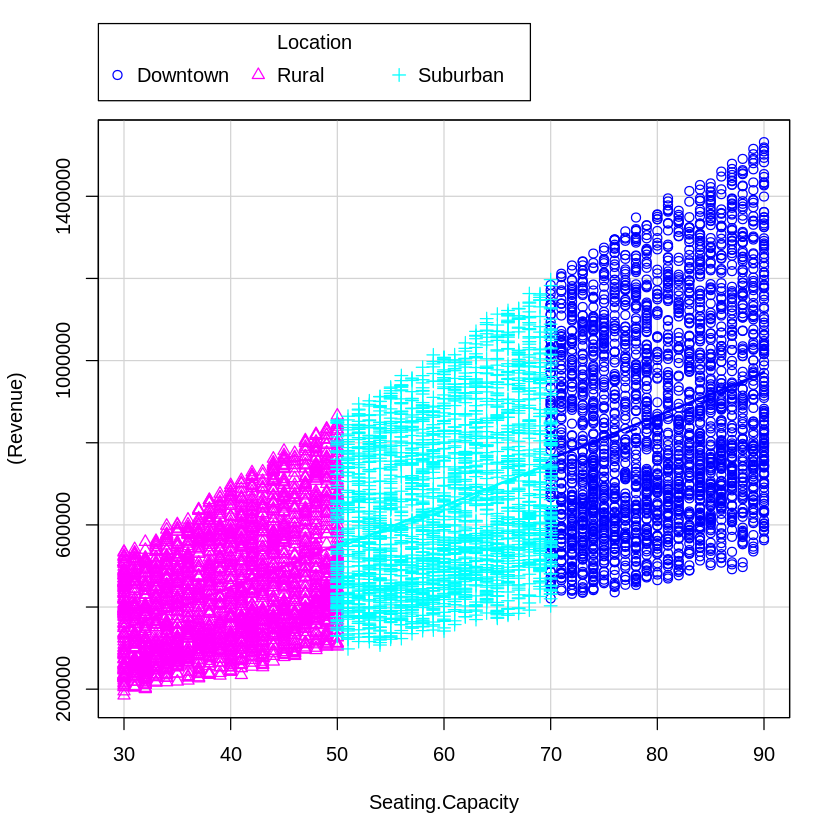
\includegraphics[width=.4\linewidth]{img/revBySeatGroupLocation.png}
\end{subfigure}
\caption{Scatterplot: Revenue by SeatingCapacity grouped by Location and AverageMealPrice grouped by Cuisine}
\label{fig:scaled_revenue_distribution_seatingcapacity_location}
\end{figure}
Therefore, we will add this in the model for further checking.

\subsubsection{Transformation of Average Meal Price}

We examine the Box Cox plot of weight:

\begin{figure}[H]
\centering
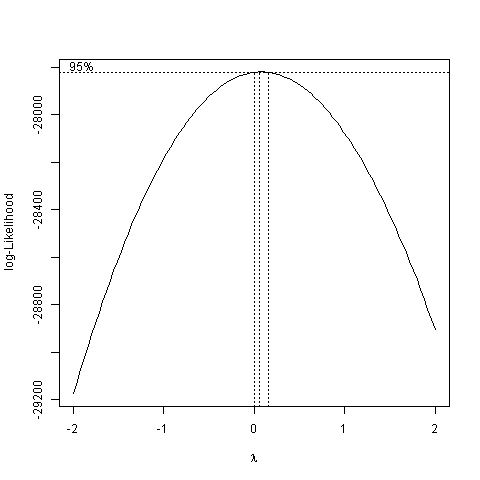
\includegraphics[scale=0.4]{img/Averboxcox.png}
\label{fig:my_label_with_H}
\caption{Box Cox plot of Average Meal Price}
\end{figure}

As Average Meal Price box cox interval is almost 0. We decide to apply the log transformation to it.

\subsubsection{Result model}

From the previous section, we have the new model:
\begin{center}
$
Revenue \ = \beta_0 + \beta_1 \left(\text{SeatingCapacity} \times \log(\text{AverageMealPrice})\right) + \beta_2 \left(\text{SeatingCapacity} \times \text{Location}\right) + \beta_3 \left(\log(\text{AverageMealPrice}) \times \text{Cuisine}\right) + \beta_4 \sqrt{\text{WeekdayReservations}} + \beta_5 \sqrt{\text{WeekendReservations}} + \epsilon
$
\end{center}

Putting this model through stepwise procedure we got the same model.

\begin{table}[ht]
\centering
\captionof{table}{Restaurant model summary}
\begin{tabular}{rrrrr}
  \hline
 & Estimate & Std. Error & t value & Pr($>$$|$t$|$) \\ 
  \hline
(Intercept) & -148660.8591 & 5420.5851 & -27.43 & 0.0000 \\ 
  sqrt(Weekday.Reservations) & -647.7837 & 316.8199 & -2.04 & 0.0409 \\ 
  sqrt(Weekend.Reservations) & -842.6644 & 323.4639 & -2.61 & 0.0092 \\ 
  Seating.Capacity:log(Average.Meal.Price) & 3110.1851 & 18.1174 & 171.67 & 0.0000 \\ 
  Seating.Capacity:LocationRural & 984.2925 & 69.6286 & 14.14 & 0.0000 \\ 
  Seating.Capacity:LocationSuburban & 285.8088 & 30.4116 & 9.40 & 0.0000 \\ 
  log(Average.Meal.Price):CuisineFrench & 47357.0901 & 515.9533 & 91.79 & 0.0000 \\ 
  log(Average.Meal.Price):CuisineIndian & -10379.0297 & 587.1932 & -17.68 & 0.0000 \\ 
  log(Average.Meal.Price):CuisineItalian & 24025.5973 & 535.5268 & 44.86 & 0.0000 \\ 
  log(Average.Meal.Price):CuisineJapanese & 69096.7374 & 514.4629 & 134.31 & 0.0000 \\ 
  log(Average.Meal.Price):CuisineMexican & -21938.8074 & 626.6495 & -35.01 & 0.0000 \\ 
   \hline
\end{tabular}
\\
Multiple R-squared:  0.9659 \\
Adjusted R-squared:  0.9659 \\
\end{table}

Hence, we check the error normality assumption of this resulting model and our baseline.

\begin{table}[H]
\centering
\captionof{table}{Shapiro-Wilk test result}
\begin{tabular}{lll}
  \hline
         &       W             & p-value    \\
    \hline
        Baseline & 0.98703 & 4.078e-11
        Improved model & 0.99837 & 0.1033 \\
   \hline
\end{tabular}
\label{tab:vif}
\end{table}

So our new model preserve the error normality assumption.

\subsection{Hypothesis testing}

Before proceeding, we rewrite our model a little bit:

\begin{center}
$
M: \ Revenue \ = \beta_0 + \beta_1 \left(\text{SeatingCapacity} \times \log(\text{AverageMealPrice})\right) + \beta_2 \left(\text{SeatingCapacity} \times \text{Location}\right) + \beta_3 \left(\log(\text{AverageMealPrice}) \times \text{Cuisine}\right) + \beta_4 \sqrt{\text{WeekdayReservations}} + \beta_5 \sqrt{\text{WeekendReservations}} + \epsilon
$
\end{center}

\subsubsection{Model utility}

We are testing the hypothesis:

\begin{center}
    $H_0: \beta_i = 0, i \in \{1,2,3,4,5\}$
    $ \\ $
    $H_1:$ At least one of $\beta_i \neq 0, i \in \{1,2,3,4,5\}$
\end{center}

This mean we are calculating the test statistic value $f= \frac{R^2/k}{1-R^2} \ \frac{1}{(n-(k+1)}$.

Based on the results of your linear regression model, the F-statistic is \( F = 18{,}930 \), which corresponds to a p-value of less than \( 2.2 \times 10^{-16} \). This extremely low p-value indicates that we can confidently reject the null hypothesis (\( H_0 \)) that all the coefficients are zero. Therefore, we can conclude that the model contains a significant linear relationship between the response variable \texttt{Revenue} and at least one of the predictor variables included in the model.


\subsubsection{Error normality assumption}

We are testing the hypothesis of:

\begin{center}
    \( H_0: \epsilon \) is normally distributed \\
    \( H_1: \epsilon \) is not normally distributed
\end{center}

To test this, we can use the test data. Let \texttt{predict\_revenue} be our result after passing the test observation through the model. Let \texttt{revenue} be the corresponding value of that observation. Then, \( \epsilon = \texttt{predict\_revenue} - \texttt{revenue} \). We will run the Shapiro-Wilk test on this resulting error.

Here is the result of our Shapiro-Wilk test:

\begin{table}[H]
\centering
\captionof{table}{Shapiro-Wilk test result}
\begin{tabular}{ll}
  \hline
                W             & p-value    \\
  \hline
        0.99837   & 0.1033   \\
  \hline
\end{tabular}
\label{tab:shapiro}
\end{table}

This means we have failed to reject the hypothesis that \( \epsilon \) is normally distributed.

\subsubsection{Autocorrelation}

We are testing the hypothesis:

\begin{center}
    \( H_0: \) There is no autocorrelation in the error terms of the linear regression model. \\
    \( H_1: \) There is autocorrelation in the error terms of the linear regression model.
\end{center}

To test this, we can run the Durbin-Watson test, which is available in R. After running the test, we get the result:

\begin{table}[H]
\centering
\captionof{table}{Durbin-Watson test result}
\begin{tabular}{ll}
  \hline
                D-W Statistic & p-value    \\
  \hline
        2.012079           & 0.598   \\
  \hline
\end{tabular}
\label{tab:durbin-watson}
\end{table}

This means we have failed to reject the null hypothesis. This indicates that there is no significant autocorrelation in the error terms of the linear regression model.

\subsection{Validation and testing}

We used the same definition of predict$\_$revenue as the previous section. It's the result of passing the test data through our model.

Here is the histogram of predict$\_$revenue:


\begin{figure}[H]
\centering
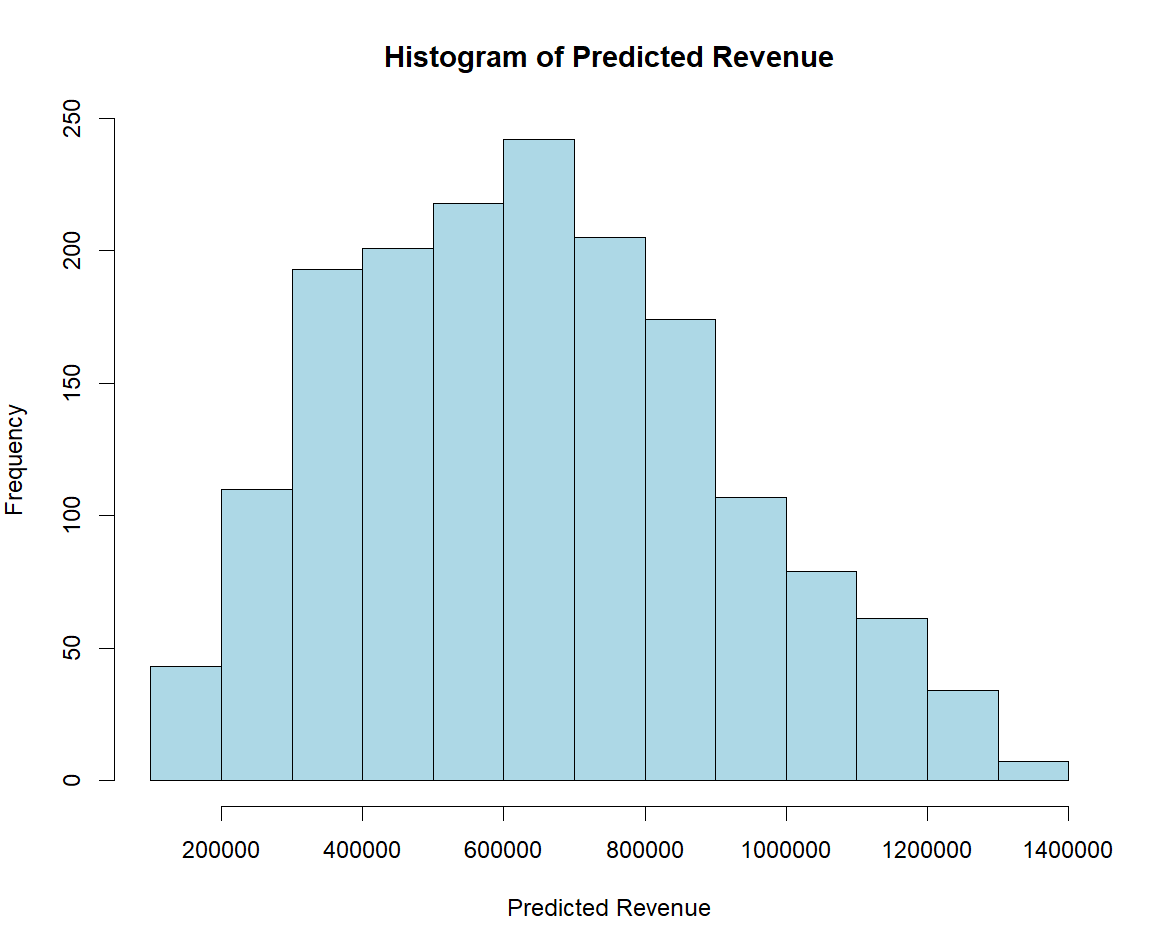
\includegraphics[width=0.7\textwidth]{img/h1b21.png}
\label{fig:scaled_revenue_distribution}
\end{figure}

We compare this to revenue, here is the scatter plot of them:

\begin{figure}[H]
\centering
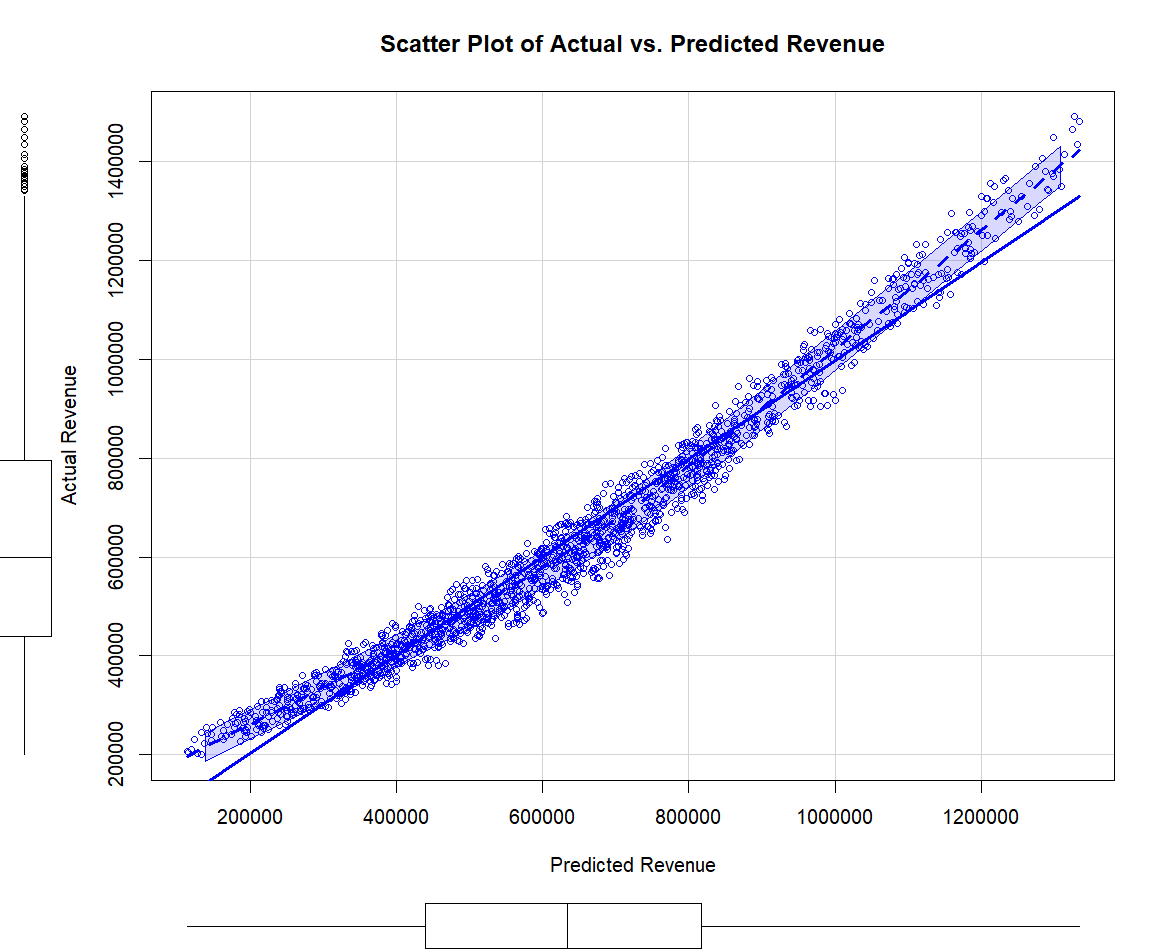
\includegraphics[width=0.7\textwidth]{img/h2b21.png}
\label{fig:scaled_revenue_distribution}
\end{figure}

As they form a almost 45 degree line in the diagonal of the graph, we can say that our model have predict the value of revenue pretty closely.



\subsection{Model Meaning}

Our model is designed to estimate restaurant revenue based on various factors, including seating capacity, meal price, location, cuisine type, and reservation data. The following is our final model:

\begin{center}
$
M: \ \text{Revenue} \ = \ \beta_1 \ + \ \beta_2 \sqrt{\text{Weekday Reservations}} \ + \ \beta_3 \sqrt{\text{Weekend Reservations}} \ + \ \beta_4 \ \text{Seating Capacity} \times \log(\text{Average Meal Price}) \ + \ \beta_5 \ \text{Seating Capacity} \times \text{Location} \ + \ \beta_6 \ \log(\text{Average Meal Price}) \times \text{Cuisine} \ + \ \epsilon
$
\end{center}

With:

\begin{center}
    $\beta_1 = -148660.86$ \\
    $\beta_2 = -647.78$ \\
    $\beta_3 = -842.66$ \\
    $\beta_4 = 3110.19$ \\
    $\beta_5 = \text{Varies by Location}$ \\
    $\beta_6 = \text{Varies by Cuisine}$
\end{center}

Variable Definitions:

\begin{itemize}
    \item Revenue: The restaurant's total revenue.
    \item Weekday Reservations: Number of reservations made during weekdays.
    \item Weekend Reservations: Number of reservations made during weekends.
    \item Seating Capacity: The number of seats available in the restaurant.
    \item Average Meal Price: The average price of a meal at the restaurant.
    \item Location: The location of the restaurant (Urban, Suburban, or Rural).
    \item Cuisine: The type of cuisine served by the restaurant (e.g., French, Indian, Italian, etc.).
\end{itemize}

Key Takeaways:

\begin{itemize}
    \item The initial revenue intercept is -148660.86.
    \item An increase in weekday or weekend reservations tends to decrease revenue slightly.
    \item Larger seating capacity combined with higher meal prices significantly increases revenue.
    \item Location impacts revenue, with rural locations having a higher effect than suburban ones.
    \item The type of cuisine influences the impact of meal price on revenue, with Japanese cuisine showing the highest positive effect.
\end{itemize}

In layman's terms:

\begin{itemize}
    \item Restaurants with more seats and higher-priced meals tend to earn more revenue.
    \item Weekday and weekend reservations slightly reduce revenue, possibly due to operational costs.
    \item Rural restaurants generally have higher revenue compared to suburban ones, when all other factors are the same.
    \item Japanese cuisine is the most lucrative when combined with higher meal prices.
\end{itemize}

Please note that these conclusions are drawn from the dataset used and may not fully represent real-world dynamics. However, within the scope of our data, the model provides accurate estimates of restaurant revenue.

%\section{Question 2: Dataset 2}

%Something here

\subsection{Data Preproccessing}

First of all, we import data from the day.csv file.
The dataset contains 731 observations with 16 columns, including factors such as weather conditions, seasonal information, temperature, and rental counts.

Dataset Overview Date Range: The data spans from January 1, 2011, to December 31, 2012.
Key Variables: season : season (1:springer, 2:summer, 3:fall, 4:winter) workingday : if day is neither weekend nor holiday is 1, otherwise is 0.
temp: Normalized temperature in Celsius.
atemp: Normalized feeling temperature in Celsius.
hum: Normalized humidity.
windspeed: Normalized wind speed.
casual: Count of casual users.
registered: Count of registered users.
cnt: Total count of bike rentals (sum of casual and registered).

In this report, we choose to analyze the relationship between total number of rentals due to environment settings.
Therefore we will skip the following collumn: instant, date


\begin{table}[ht]
\centering
\begin{tabular}{lllllrrrrrr}
  \hline
  season & holiday & weekday & workingday & weathersit & temp & atemp & hum & windspeed & registered & cnt \\ 
  \hline
 1 & 0 & 4 & 1 & 2 & 0.40 & 0.40 & 0.67 & 0.19 & 3571 & 3761 \\ 
   4 & 0 & 5 & 1 & 1 & 0.36 & 0.36 & 0.54 & 0.21 & 5283 & 5992 \\ 
   2 & 0 & 1 & 1 & 1 & 0.53 & 0.53 & 0.59 & 0.18 & 3698 & 4362 \\ 
   2 & 0 & 3 & 1 & 2 & 0.62 & 0.58 & 0.77 & 0.10 & 4494 & 5260 \\ 
   2 & 0 & 0 & 0 & 1 & 0.61 & 0.57 & 0.51 & 0.23 & 4286 & 7132 \\ 
   4 & 0 & 3 & 1 & 2 & 0.48 & 0.47 & 0.72 & 0.15 & 3490 & 3894 \\ 
   \hline
\end{tabular}
\end{table}

\subsubsection{Missing data}

According to the author description, there is no missing value in this dataset, so it is not a problem that we should care for.

\subsubsection{Dependent variables choosing}

Because of a few factors, we chose to use registered as our dependent variable: registered is one of the 3 dependent variables that we can choose and all other variables yr, season, holiday, workingday, weathersit, mnth have some relation with registered in an acceptable level.

\subsubsection{Outlier}

\begin{figure}[H]
\centering
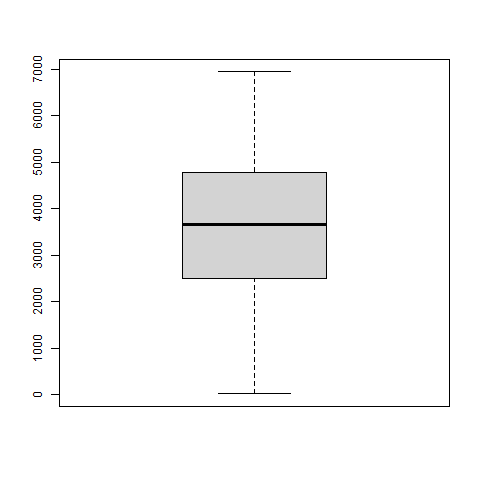
\includegraphics[scale=.4]{img/registered_box_plot.png}
\caption{Box plot of registered}
\label{fig:registered_box_plot}
\end{figure}

Looking at the box plot, we can see that there is no outliers for our dependent variable.

\subsection{Data overview}
First of all, we might want to look at the summary table contain the statistic descriptive to have the overview about our dataset.

\begin{table}[ht]
\centering
\begin{tabular}{lllllll}
  \hline
         &      temp &     atemp &      hum &   windspeed &   registered &      cnt \\ 
  \hline
      Min& 0.05913& 0.07907& 0.0000& 0.02239& 20& 22\\ 
        1st Qu.& 0.33708& 0.33784& 0.5200& 0.13495& 2497& 3152\\ 
          Median& 0.49833& 0.48673& 0.6267& 0.18097& 3662& 4548\\ 
          Mean& 0.49538& 0.47435& 0.6279& 0.19049& 3656& 4504\\ 
           3rd Qu.& 0.65542& 0.60860& 0.7302& 0.23321& 4776& 5956\\ 
           Max& 0.86167& 0.84090& 0.9725& 0.50746& 6946& 8714\\ 
            &  &  &  &  &  &  \\ 
   \hline
\end{tabular}
\end{table}


\subsubsection{Key Observations:}

\begin{itemize}
    \item \textbf{Variation}: The continuous variables show significant variation, particularly \textbf{humidity} and \textbf{windspeed}.
    \item \textbf{Central Tendency}: The mean and median values for most variables are close, indicating a relatively symmetrical distribution.
    \item \textbf{Range}: The wide range in values for \textbf{registered} indicates days with both low and high rental counts.
\end{itemize}
This summary provides a good foundation for further analysis, such as examining relationships between variables or identifying potential outliers.

 


\subsection{Data deepdive}
To have a deeper look about our dataset and how the variable actually related with each other, we will have to look at the correlation heatmap plot, which was conducted to identify relationships between numeric variables

\begin{figure}[H]
\centering
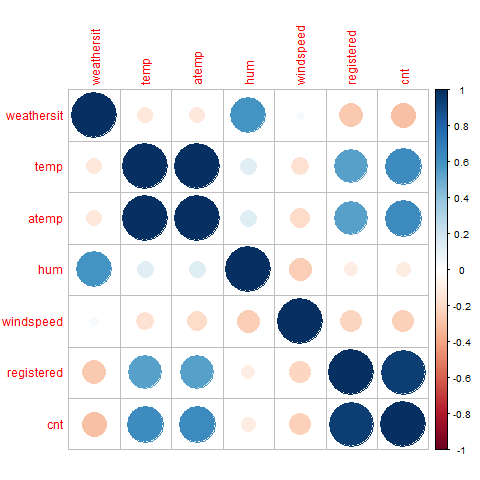
\includegraphics[width=0.7\textwidth]{img/corplot.png}
\caption{Correlation Matrix}
\label{fig:Correlation_matrix_Q2_2}
\end{figure}

We can observe that there is a strong correlation in some variables, especially between temp and atemp.

\subsection{Data splitting}

The data is split into two part, training dataset and validation dataset. Training dataset contains 80$\%$ of the observations and the validation dataset contains 80$\%$ of the observations. The split is performed randomly with RStudio.

For replication, we use the seed 777489.

\subsection{Building baseline model}

From the above section we can see that temp and atemp have a strong relationship. Below is a plot that describe how much the relation is:

\begin{figure}[H]
\centering
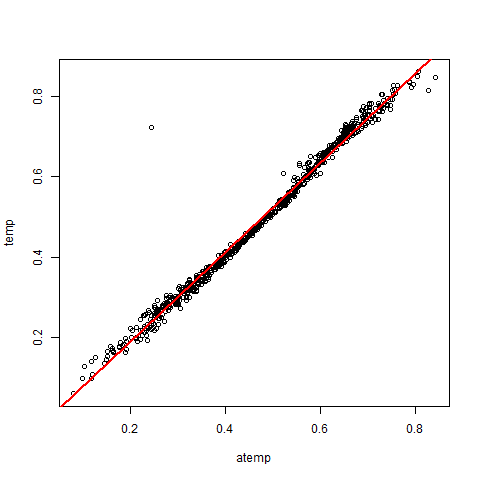
\includegraphics[width=0.7\textwidth]{img/temp_atemp.png}
\caption{Relation between temp and atemp}
\label{fig:relation_between_temp_and_atemp}
\end{figure}


As we can see from the plot, temp and atemp have a strong linear relationship. Therefore, we will not use atemp in our model.

In our decription, holiday and workingday and weekday also have strong relation. If it is a holiday then it is not a working day and weekday is 6 it also not a workingday.  

To choose which one we will include in our baseline model, we look on how much they impact to the registered through box-plot.

\begin{figure}[H]
\centering
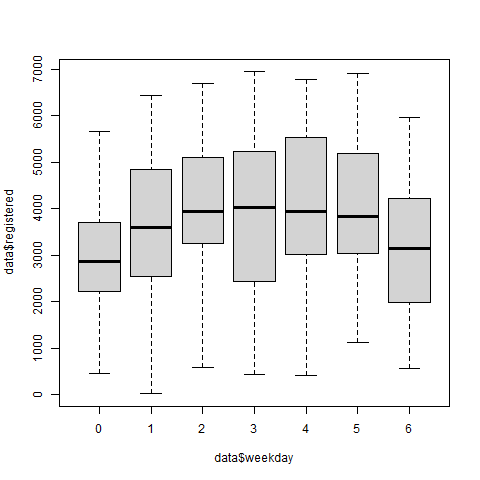
\includegraphics[width=0.55\textwidth]{img/weekday.png}
\caption{Impact of Weekday}
\label{fig:scaled_revenue_distribution}
\end{figure}

\begin{figure}[H]
\centering
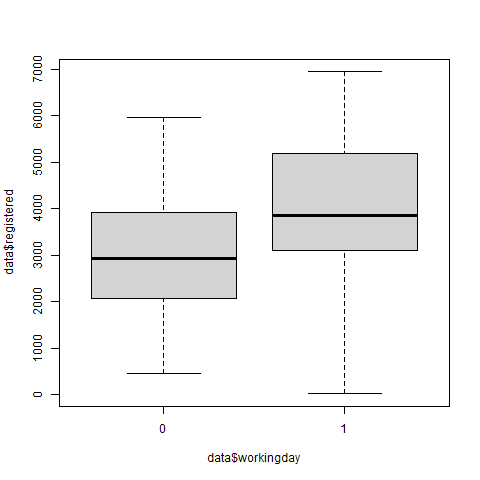
\includegraphics[width=0.55\textwidth]{img/workingday.png}
\caption{Impact of Workingday}
\label{fig:scaled_revenue_distribution}
\end{figure}

\begin{figure}[H]
\centering
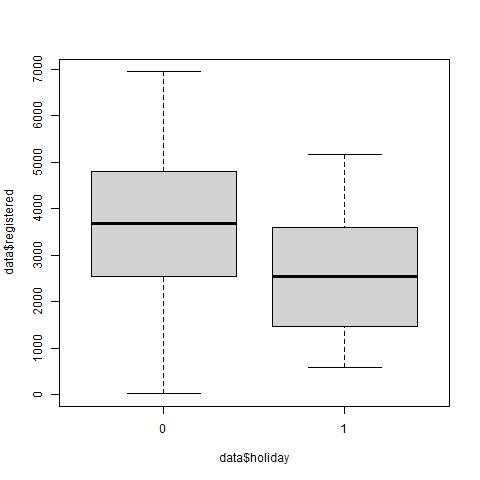
\includegraphics[width=0.55\textwidth]{img/holiday.png}
\caption{Impact of holiday}
\label{fig:scaled_revenue_distribution}
\end{figure}

From the definition, we can clearly figure out that when weekday is 0 or 6, working day is 0, this lead to multicollinearity. Consider that the impact of the weekday is not more significant than the other two, we decide not to use this variable in out model.

temp:
\begin{figure}[H]
\centering
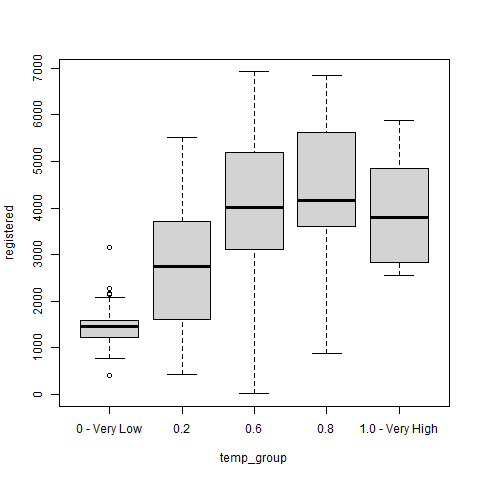
\includegraphics[width=0.55\textwidth]{img/plottemp3.png}
\caption{Impact of temp}
\label{fig:scaled_revenue_distribution}
\end{figure}

People tend to use rental bicycles more when temperature is warmer but not too hot. 

Humidity:
\begin{figure}[H]
\centering
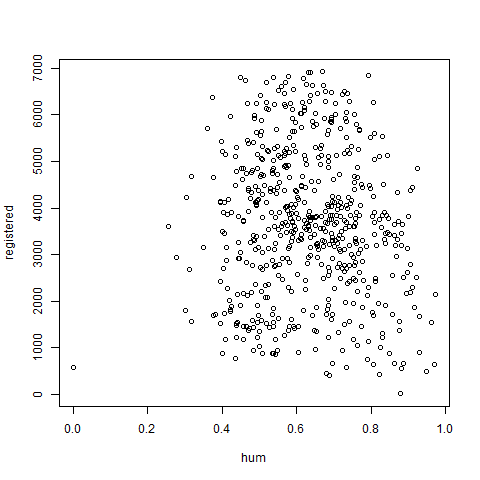
\includegraphics[width=0.55\textwidth]{img/plothum.png}
\caption{Plot of how registered depend on humidity}
\label{fig:humidity_on_registered_plot}
\end{figure}

As we can see, most of the data collected is in range [0.4,0.8] and humidity is clearly have relation on registered, so we are going to keep it.

Similarly, we will keep windspeed, season and yr, mnth (we may want to eliminate them later)
We have our first baseline model

\begin{center}
    $registered = \beta_1 \ + \ \beta_2 \ holiday \ + \ \beta_3 \ yr \ + \ \beta_{4,i} \ mnth_i \ + \ \beta_{5,j} \ weathersit_j \ + \ \beta_6 \ temp \ + \ \beta_7 \ hum \ + \ \beta_8 \ windspeed \ + \ \beta_{9,k} \ season_k$
\end{center}

\subsubsection{Splitting data}

 set.seed(777489)
Randomly, we choose 777489 as seed

We will split 80-20, 80 for the training dataset and 20 for test dataset



\subsection{Improving to a better model}

Currently, our baseline model is in the form:

\begin{center}
    $registered = \beta_1 \ + \ \beta_2 \ holiday \ + \ \beta_3 \ yr \ + \ \beta_{4,i} \ mnth_i \ + \ \beta_{5,j} \ weathersit_j \ + \ \beta_6 \ temp \ + \ \beta_7 \ hum \ + \ \beta_8 \ windspeed \ + \ \beta_{9,k} \ season_k$
\end{center}

With:

\begin{center}
    $i \in \{2,3,...,12\}$
    \\
    $j \in \{2,3\}$
    \\
    $k \in \{1,2,3\}$
\end{center}

\subsubsection{Inspection of interaction terms}
In order to improve the model, we inspect the interaction between qualitative and quantitative variables to determine which interactions impact the response. Using scatter plots, we draw and inspect all combinations between a qualitative variable with a quantitative variable. After all combinations have been tested with, we end up with 4 pairs of indicators that has a relationship with the response.  

\begin{figure}[H]
\centering
%\includegraphics[scale=.4]{Insert scatter plot pls}
\caption{Scatter plot showing the interaction of indicators influencing the response}
\label{fig:scattplot_with 4}
\end{figure}
\subsubsection{Adding the interaction terms into the model}
We then adding the interaction terms into the model firstly by removing all the qualitative terms that appears in the interaction terms and then adding all the interaction terms into the model. The new model, while having decent adjusted $R^2$ value, fails to pass the Shapiro-Wilk test with significance level 0.05 when tested with test data.

Then, from the removed quantitative terms, we check to see if adding any subset of them into the model improve the outcome. The results show that only the subset of the 'weathersit' term improve the model enough to pass the Shapiro-Wilk test while still having decent $R^2$ value. 

\subsubsection{The improved model}

From various adjustment from the previous sections, we are now left with our new model:

\begin{center}
    $registered = \beta_1 \ + \ \beta_2 \ holiday \ + \ \beta_3 \ yr \ + \ \beta_{4,i} \ (temp \times mnth_i) \ + \ \beta_{5,i} \ (hum \times mnth_i) \ + \ \beta_{6,j} \ (hum \times weathersit_j) \ + \ \beta_{7,k} \ (temp \times season_k) \ + \ \beta_{8,j} \ weathersit_j \ + \ \beta_9 \ temp \ + \ \beta_{10} \ hum \ + \ \beta_{11} \ windspeed$
\end{center}

\begin{table}[H]
\centering
\captionof{table}{Summary of the new model}
\begin{tabular}{rrrrr}
  \hline
 & Estimate & Std. Error & t value & Pr($>$$|$t$|$) \\ 
  \hline
(Intercept) & 1145.0924 & 256.8485 & 4.46 & 0.0000 \\ 
  weekday1 & -276.9376 & 170.9994 & -1.62 & 0.1059 \\ 
  weekday2 & -40.7826 & 185.5718 & -0.22 & 0.8261 \\ 
  weekday3 & -48.8690 & 185.8878 & -0.26 & 0.7927 \\ 
  weekday4 & 36.9159 & 184.6410 & 0.20 & 0.8416 \\ 
  weekday5 & -77.5401 & 184.0552 & -0.42 & 0.6737 \\ 
  weekday6 & 268.8323 & 94.4005 & 2.85 & 0.0046 \\ 
  workingday1 & 1142.0029 & 161.2402 & 7.08 & 0.0000 \\ 
  yr & 1713.6644 & 54.1621 & 31.64 & 0.0000 \\ 
  weathersit2 & 687.6415 & 368.8965 & 1.86 & 0.0629 \\ 
  weathersit3 & -562.2423 & 4012.8893 & -0.14 & 0.8886 \\ 
  temp & 2949.3213 & 1055.1483 & 2.80 & 0.0054 \\ 
  hum & -1475.3014 & 554.5679 & -2.66 & 0.0080 \\ 
  windspeed & -1794.6719 & 370.5045 & -4.84 & 0.0000 \\ 
  temp:season2 & 2283.9905 & 407.7851 & 5.60 & 0.0000 \\ 
  temp:season3 & 2504.4678 & 440.2888 & 5.69 & 0.0000 \\ 
  temp:season4 & 3621.3753 & 453.9504 & 7.98 & 0.0000 \\ 
  temp:mnth2 & -394.2637 & 1310.5266 & -0.30 & 0.7636 \\ 
  temp:mnth3 & 289.4883 & 1305.9652 & 0.22 & 0.8247 \\ 
  temp:mnth4 & -813.6620 & 1263.2824 & -0.64 & 0.5198 \\ 
  temp:mnth5 & -2917.4178 & 1313.2722 & -2.22 & 0.0267 \\ 
  temp:mnth6 & -2330.3152 & 1294.6958 & -1.80 & 0.0724 \\ 
  temp:mnth7 & -4711.1287 & 1255.5836 & -3.75 & 0.0002 \\ 
  temp:mnth8 & -2009.8108 & 1379.9392 & -1.46 & 0.1458 \\ 
  temp:mnth9 & 16.0030 & 1427.8247 & 0.01 & 0.9911 \\ 
  temp:mnth10 & -305.6074 & 1423.1634 & -0.21 & 0.8301 \\ 
  temp:mnth11 & -1701.7563 & 1733.2287 & -0.98 & 0.3266 \\ 
  temp:mnth12 & 1919.7097 & 1745.4852 & 1.10 & 0.2719 \\ 
  hum:mnth2 & 360.2283 & 605.7862 & 0.59 & 0.5523 \\ 
  hum:mnth3 & 347.2989 & 695.7390 & 0.50 & 0.6179 \\ 
  hum:mnth4 & 360.2651 & 634.4346 & 0.57 & 0.5704 \\ 
  hum:mnth5 & 2139.9813 & 744.6248 & 2.87 & 0.0042 \\ 
  hum:mnth6 & 1713.1093 & 875.0156 & 1.96 & 0.0508 \\ 
  hum:mnth7 & 3677.8064 & 816.0531 & 4.51 & 0.0000 \\ 
  hum:mnth8 & 963.3453 & 953.7447 & 1.01 & 0.3129 \\ 
  hum:mnth9 & -24.5940 & 877.4098 & -0.03 & 0.9776 \\ 
  hum:mnth10 & 206.7723 & 747.9856 & 0.28 & 0.7823 \\ 
  hum:mnth11 & 830.5844 & 883.6153 & 0.94 & 0.3476 \\ 
  hum:mnth12 & -736.0092 & 783.1167 & -0.94 & 0.3477 \\ 
  weathersit2:hum & -1557.9168 & 544.4051 & -2.86 & 0.0044 \\ 
  weathersit3:hum & -1323.4362 & 4450.3771 & -0.30 & 0.7663 \\ 
   \hline
\end{tabular}
\\
Multiple R-squared:  0.8577 \\
Adjusted R-squared:  0.8473 \\
F-statistic: 81.85 on 40 and 543 DF,  p-value: < 2.2e-16 \\
\end{table}

We put this through the stepwise method, to our surprise, no variable is eliminated. 

Therefore, we just compare the evaluation variable to the baseline.

\begin{table}[H]
\centering
\captionof{table}{Evaluation parameter of the baseline and improved model}
\begin{tabular}{lll}
  \hline
               & Improved model             & Baseline    \\
    \hline
$R^2$          & \textbf{0.7859}    & 0.7688    \\
Adjusted $R^2$ & \textbf{0.7726}    & 0.7602    \\
AIC            & \textbf{9406.626} & 9425.379 \\
BIC            & 9563.943   & \textbf{9525.887} \\
   \hline
\end{tabular}
\label{tab:vif}
\end{table}

There are improvement in 3 out of 4 parameter. This does not assure us the improved model is better. Therefore, we use a wildcard parameter. We run the Shapiro-Wilk test on both model to check whether the error is normal distributed.

\begin{table}[H]
\centering
\captionof{table}{Shapiro-Wilk test result}
\begin{tabular}{lll}
  \hline
         &       W             & p-value    \\
    \hline
        Baseline &  0.9594 & 0.0002534   \\
        Improved model & 0.9837 & 0.07929 \\
   \hline
\end{tabular}
\label{tab:vif}
\end{table}

So the result of the test indicate that the error for the improved model is more likely to be normal distributed. Hence, we decide to pick this as our final model.
\subsection{Hypothesis testing}

Before proceeding, we rewrite our model a little bit:

\begin{center}
    $registered = \beta_1 \ + \ \beta_2 \ holiday \ + \ \beta_3 \ yr \ + \ \beta_{4,i} \ (temp \times mnth_i) \ + \ \beta_{5,i} \ (hum \times mnth_i) \ + \ \beta_{6,j} \ (hum \times weathersit_j) \ + \ \beta_{7,k} \ (temp \times season_k) \ + \ \beta_{8,j} \ weathersit_j \ + \ \beta_9 \ temp \ + \ \beta_{10} \ hum \ + \ \beta_{11} \ windspeed$
\end{center}
\subsubsection{Model utility}

We are testing the hypothesis:

\begin{center}
    $H_0: \beta_i = 0, i \in \{2,3,4,5,6,7,8,9,10,11\}$
    $ \\ $
    $H_1:$ At least one of $\beta_i \neq 0, i \in \{2,3,4,5,6,7,8,9,10,11\}$
\end{center}

This mean we are calculating the test statistic value $f= \frac{R^2/k}{1-R^2} \ \frac{1}{(n-(k+1)}$.

Plugging in the number we get $f = 81.85$, this corresponding to a p-value of $2,2.10^{-16}$. This mean we can be certain to reject $H_0$. And conclude that our model contains useful linear relationship between our the response \texttt{Registered} and at least one of the variable.
\subsubsection{Error normality assumption}

We are testing the hypothesis of:

\begin{center}
    $H_0: \epsilon$ is normal distributed
    \\
    $H_1:\epsilon$ is not normal distributed
\end{center}

To test this, we can use the test data. Let's $predict\_registred$ be our result after passing the test observation through the model. Let's mpg be the corresponding value of that observation. Then, $\epsilon = predict\_registered - registered$. We will run the Shapiro-Wilk test through this resulting error.

Here the result of our Shapiro-Wilk test:

\begin{table}[H]
\centering
\captionof{table}{Shapiro-Wilk test result}
\begin{tabular}{ll}
  \hline
                W             & p-value    \\
    \hline
        0.9837& 0.07929\\

   \hline
\end{tabular}
\label{tab:vif}
\end{table}

This mean we have failed to reject the hypothesis that $\epsilon$ is normal distributed. 

\subsubsection{Homoskedastic residual variance}

Here we are testing the hypothesis of:

\begin{center}
    $H_0:$ The residuals variances of the groups are equal.
    \\
    $H_1:$ At least one group has a different residuals variance.
\end{center}

To test this, we can run the Levene's test, which is available in R. After running the test, we get the result:

\begin{table}[H]
\centering
\captionof{table}{Levene test result}
\begin{tabular}{ll}
  \hline
                F             & p-value    \\
    \hline
        3.392 &  0.06602   \\

   \hline
\end{tabular}
\label{tab:vif}
\end{table}

This mean we have failed to reject the null hypothesis. This indicate that the residuals variances of the groups are equal.

\subsubsection{Autocorrelation}

We are testing the hypothesis:

\begin{center}
    $H_0:$ There is no autocorrelation in the error terms of the linear regression model.
    \\
    $H_1:$ There is positive autocorrelation in the error terms of the linear regression model.
\end{center}

To test this, we can run the Durbin-Watson test, which is available in R. After running the test, we get the result:

\begin{table}[H]
\centering
\captionof{table}{Durbin-Watson test result}
\begin{tabular}{ll}
  \hline
                D-W             & p-value    \\
    \hline
        2.061362  & 0.47   \\

   \hline
\end{tabular}
\label{tab:vif}
\end{table}

This mean we have failed to reject the null hypothesis. This indicate that there is no autocorrelation in the error terms of the linear regression model.

\subsection{Validation and testing}

We used the same definition of predict$\_$registered as the previous section. It's the result of passing the test data through our model.

Here is the histogram of predict$\_$registered:


\begin{figure}[H]
\centering
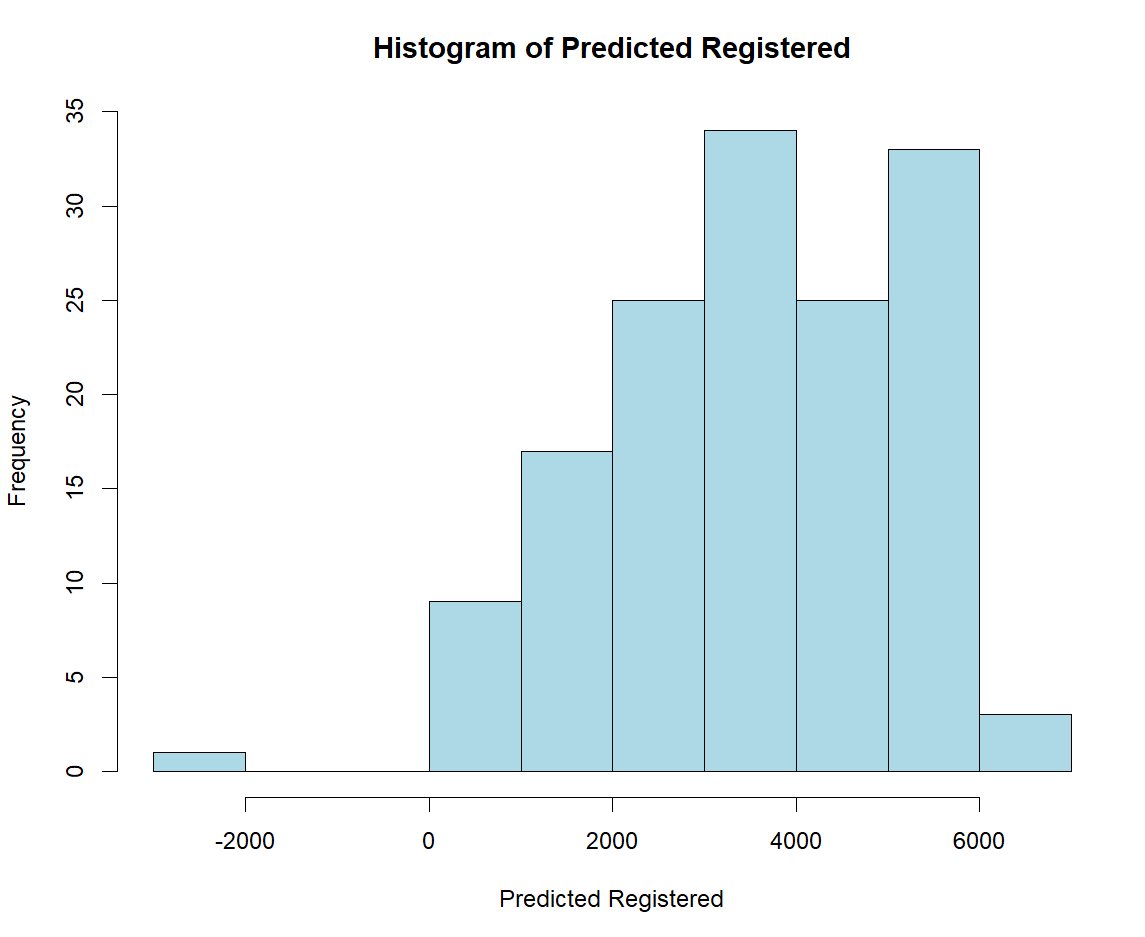
\includegraphics[width=0.7\textwidth]{img/h1b22.png}
\label{fig:scaled_revenue_distribution}
\end{figure}

We compare this to registered, here is the scatter plot of them:

\begin{figure}[H]
\centering
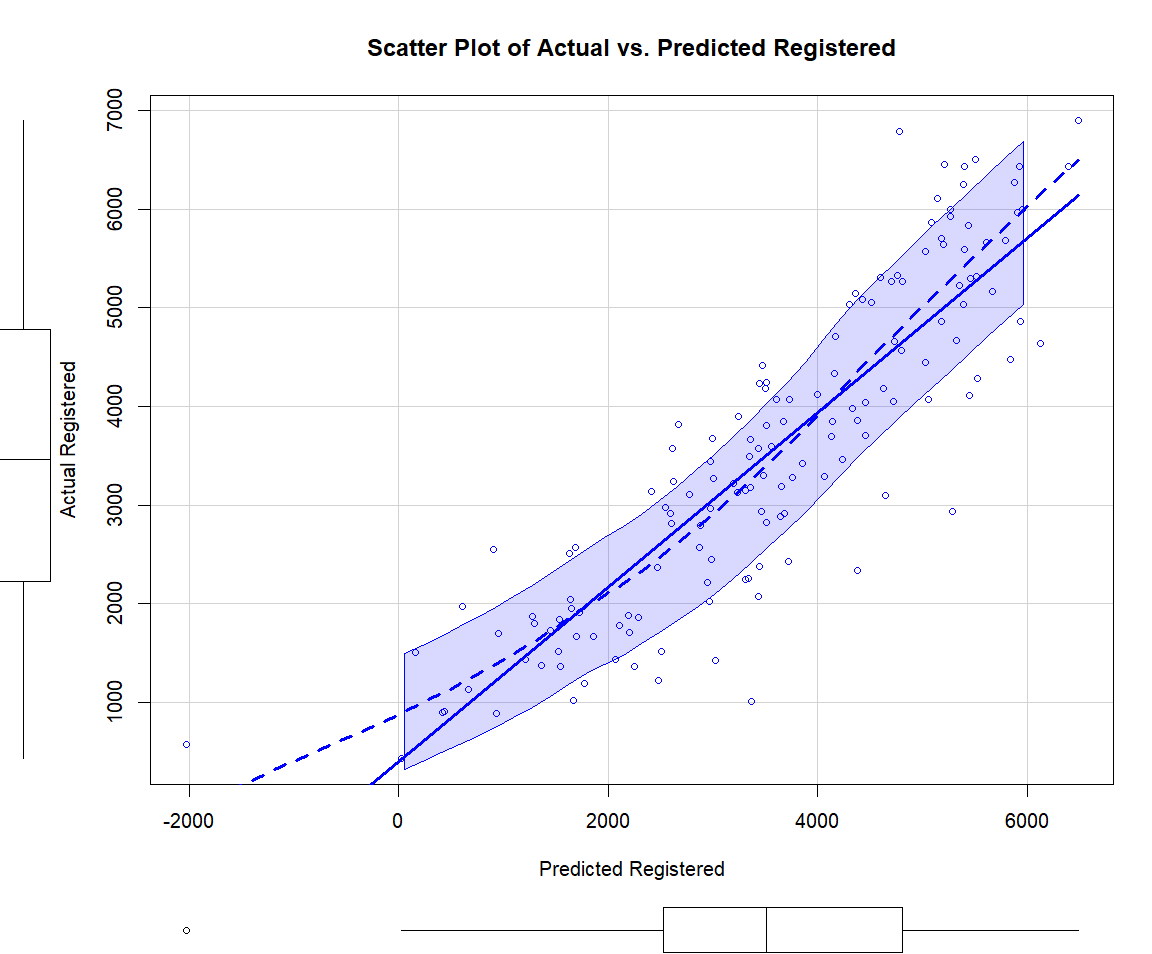
\includegraphics[width=0.7\textwidth]{img/h2b22.png}
\label{fig:scaled_revenue_distribution}
\end{figure}

As they form a almost 45 degree line in the diagonal of the graph, we can say that our model have predict the value of mpg pretty closely.

\subsection{Model Meaning}

Our model is capable of estimating the number of registered bike rentals based on several parameters: holiday, year, weather situation, temperature, humidity, windspeed, and their interactions with month and season. Since the year is used as a continuous variable, this model can also be used for future predictions, though the accuracy may need to be reexamined for future years.

Overall, here is our final model:

\begin{center}
$
M: \ registered \ = \ \beta_1 \ + \ \beta_2 \ holiday \ + \ \beta_3 \ yr \ + \ \beta_{4, j} \ weathersit_j \ + \ \beta_5 \ temp \ + \ \beta_6 \ hum \ + \ \beta_7 \ windspeed \ + \ \beta_{8, k} \ (temp \times season_k) \ + \ \beta_{9, i} \ (temp \times mnth_i) \ + \ \beta_{10, i} \ (hum \times mnth_i) \ + \ \beta_{11, j} \ (hum \times weathersit_j) \ + \ \epsilon
$
\end{center}

With:

\begin{center}
    \begin{align*}
    \beta_1 & = 1727.34 \\
    \beta_2 & = -954.56 \\
    \beta_3 & = 1717.52 \\
    \beta_4 & = 
        \begin{cases} 
          1253.98 & \text{(weathersit2)} \\
          -4887.25 & \text{(weathersit3)} 
        \end{cases} \\
    \beta_5 & = 2806.06 \\
    \beta_6 & = -1103.72 \\
    \beta_7 & = -1923.17 \\
    \beta_8 & = 
        \begin{cases} 
          2377.63 & \text{(temp $\times$ season2)} \\
          2734.72 & \text{(temp $\times$ season3)} \\
          3958.73 & \text{(temp $\times$ season4)} 
        \end{cases} \\
    \beta_9 & = \text{varies by month (temp $\times$ mnth)} \\
    \beta_{10} & = \text{varies by month (hum $\times$ mnth)} \\
    \beta_{11} & = \text{varies by weather situation (hum $\times$ weathersit)} \\
    \end{align*}
\end{center}

Variable meanings:

\begin{itemize}
    \item registered: Number of registered bike rentals.
    \item holiday: 1 if the day is a holiday, 0 otherwise.
    \item yr: Year (0 for 2011, 1 for 2012).
    \item weathersit: Categorical variable representing the weather situation.
    \item temp: Normalized temperature in Celsius.
    \item hum: Normalized humidity.
    \item windspeed: Normalized windspeed.
    \item season: Categorical variable representing the season.
    \item mnth: Categorical variable representing the month.
\end{itemize}

This means that:

\begin{itemize}
    \item The base number of registered bike rentals, when all other variables are at their base levels, is 1727.34.
    \item If the day is a holiday, the number of registered rentals decreases by 954.56.
    \item An increase in the year variable (from 2011 to 2012) increases the number of rentals by 1717.52.
    \item Different weather situations have varying impacts, with `weathersit2` increasing rentals by 1253.98 and `weathersit3` decreasing rentals by 4887.25.
    \item As temperature increases, rentals increase by 2806.06 units.
    \item Higher humidity tends to decrease rentals, but this effect varies by month and weather situation.
    \item Higher windspeed significantly reduces the number of rentals by 1923.17 units.
    \item The interaction effects show that temperature and humidity have different impacts depending on the season, month, and weather situation.
\end{itemize}

In layman's terms, this means:

\begin{itemize}
    \item Registered bike rentals are higher in the year 2012 compared to 2011.
    \item Holidays see fewer bike rentals.
    \item Good weather (as represented by `weathersit2`) increases rentals, while bad weather (`weathersit3`) significantly reduces them.
    \item Warmer days generally lead to more bike rentals.
    \item High humidity and windspeed can decrease the number of rentals.
\end{itemize}

Please note that these conclusions are based on the dataset used and may not fully represent real-world conditions. However, within the scope of our data, the model accurately estimates the number of registered bike rentals.


%\section{Hình ảnh}
Hình ảnh được thể hiện như hình~\ref{fig:my_label}, lưu ý flag \texttt{[H]} để disable floating (hình được hiển thị đúng vị trí, không trôi lên đầu trang).
\begin{figure}%[H]
\centering

\includegraphics[scale=.4]{img/hcmus-logo.png}
\caption{Hình ví dụ (logo HCMUS - updated 30/11/2022)}
\label{fig:my_label}
\end{figure}

Hình~\ref{fig:my_label_with_H} cũng là hình ví dụ nhưng có tag \texttt{[H]}. Lưu ý là có tag \texttt{[H]} thì code ở đâu hình sẽ nằm ở đó, không quan trọng nội dung ít hay nhiều (trang giấy sẽ thừa 1 khúc như bạn thấy). Để hiểu hơn về positioning trong LaTeX, xin tham khảo \href{https://www.overleaf.com/learn/latex/Positioning_images_and_tables}{bài này}.

\begin{figure}[H]
\centering

\includegraphics[scale=.4]{img/hcmus-logo.png}
\caption{Hình ví dụ (logo HCMUS - updated 30/11/2022)}
\label{fig:my_label_with_H}
\end{figure}
%\section{Bảng biểu}
Bảng biểu được thể hiện như bảng~\ref{tab:my_label}, lưu ý flag \texttt{[H]} để disable floating (bảng được hiển thị đúng vị trí, không trôi lên đầu trang). Bảng~\ref{tab:my_label} là một trường hợp không sử dụng tag \texttt{[H]} và bảng bị trôi tít lên đầu trang:
\begin{table}%[H]
\centering
\begin{tabular}{|l|l|}
\hline
\textbf{Tên con vật} & \textbf{Số chân} \\ \hline
Gà & 2 \\ \hline
Chó & 4 \\ \hline
Trần Hoàng Tử & 2 \\ \hline
\end{tabular}
\caption{Số chân của một số con vật, không có tag \texttt{[H]}}
\label{tab:my_label}
\end{table}

Bảng~\ref{tab:my_label_with_H_tag} thể hiện bảng biểu với tag \texttt{[H]}\footnote{Tương tự cách sử dụng tag \texttt{[H]} với hình}. Để không phải mất thời gian tuổi trẻ ngồi chỉnh table, xài \href{https://www.tablesgenerator.com}{https://www.tablesgenerator.com}.

\begin{table}[H]
\centering
\begin{tabular}{|l|l|}
\hline
\textbf{Tên con vật} & \textbf{Số chân} \\ \hline
Gà & 2 \\ \hline
Chó & 4 \\ \hline
Trần Hoàng Tử & 2 \\ \hline
\end{tabular}
\caption{Số chân của một số con vật, có tag \texttt{[H]}}
\label{tab:my_label_with_H_tag}
\end{table}.
%\section{Công thức toán}
Công thức toán gõ chung 1 dòng thì dùng 2 lần dấu dollar: $f(x) = x^2 + 2x + 1$. Với công thức nằm riêng 1 dòng thì gõ 2 cặp dấu dollar:
$$
ReLU(x) = \max(0, x)
$$
Siêu việt hơn, gõ hệ phương trình thì nên dùng tag \texttt{equation}
\begin{equation*}
\begin{aligned}
a_1x_1 + a_2x_2 + .. + a_nx_n &= u \\
b_1x_1 + b_2x_2 + .. + b_nx_n &= v \\
c_1x_1 + c_2x_2 + .. + c_nx_n &= w \\
\end{aligned}
\end{equation*}
Tham khảo cách gõ equation trên \href{https://www.overleaf.com/learn/latex/Mathematical_expressions}{Overleaf} nhé!
%\section{Thuật toán}
Dùng gói \texttt{algorithm} và \texttt{algpseudocode} để gõ đoạn thuật toán~\ref{alg:label}\footnote{Tất nhiên đây là dùng katana mổ ruồi!}

\begin{algorithm}
\caption{Thuật toán đếm xem nhiều gà hay nhiều chó hơn}
\label{alg:label}
\begin{algorithmic}
\Function {GaChoSoNaoLonHon}{\textit{ga}, \textit{cho}}
\State $soGa \gets 0$
\State $soCho \gets 0$
\For {$i \in [0, |ga| - 1]$}
\State $soGa \gets soGa + 1$
\EndFor
\For {$i \in [0, |cho| - 1]$}
\State $soCho \gets soCho + 1$
\EndFor

\If {$soGa > soCho$}
\State\Return $soGa$
\ElsIf {$soGa < soCho$}
\State\Return $soCho$
\Else 
\State\Return \text{"bang nhau"}
\EndIf
\EndFunction
\end{algorithmic}
\end{algorithm}
%\section{Code}
Dùng gói \texttt{listings} để gõ code, ví dụ cho C++:
\lstinputlisting[language=C++]{code/example.cpp}

Cho Python:
\lstinputlisting[language=Python]{code/example.py}

Đặc biệt: code có comment bằng tiếng Việt
\vietnameselst
\lstinputlisting[language=Python]{code/example-vietnamese.py}
%\section{Ngôn ngữ}
Ngôn ngữ mặc định của template là Tiếng Việt, config ở file \texttt{main.tex} với lệnh
\begin{lstlisting}[language=tex]
\usepackage[utf8]{vietnam}
\end{lstlisting}
Để chuyển sang Tiếng Anh (e.g. nhiều khi bạn muốn label trong các bảng bằng Tiếng Anh; bạn muốn viết report bằng Tiếng Anh thay vì Tiếng Việt), khi đó có 2 lựa chọn:
\begin{itemize}
\item Chuyển xang xài package \texttt{babel} và xài tag \texttt{$\backslash$uselanguage}.
\item Bỏ xài package \texttt{vietnam}
\end{itemize}
Hướng dẫn thì mời bạn xem \href{https://www.overleaf.com/learn/latex/International_language_support#Babel}{link này}
%\section{Sử dụng tài liệu tham khảo}

File BibTeX tài liệu tham khảo nằm ở đường dẫn \texttt{ref/ref.bib}. Sửa tên file \texttt{.bib} sẽ phải sửa lại nội dung file \texttt{ref.tex}.

Đây là ví dụ cite một tài liệu\cite{greenwade93}.

% References
%\cleardoublepage
\phantomsection
\addcontentsline{toc}{section}{Tài liệu}
\bibliographystyle{plain}
\bibliography{ref/ref}

% Appendix
\appendix
% Add \cleardoublepage to move appendices to next page.
\section{Appendix}

\subsection{Code}

\subsubsection{Question 1}

\begin{lstlisting}
{r setup, include=FALSE}
knitr::opts_chunk$set(echo = TRUE)
Sys.setenv(LANG = "en")
setwd("C:/Users/Lecuo/Desktop/StatLabWithR")
library(dplyr)
#install.packages("xtable")
library(xtable)
#install.packages("papeR")
library(papeR)
library(car)
library(MASS)
library(ggplot2)
#install.packages("plotrix")
library(plotrix)
rm(list = ls())

data<-read.csv("auto_mpg.csv",header=TRUE,sep=';')
dim(data)
sink(file = "dataheading.txt")
data
sink(file = NULL)

data<-subset(data, data$horsepower != "?")
data$horsepower<-as.double(data$horsepower)
gooddata<-subset(data, select = -c(model_year,origin,car_name))
gooddata
xtable(summarize(gooddata), caption = "Basic univariate summary statistics for mgp, cylinders, displacement, horsepower, weight, acceleration")
sink(file = "datasummary.txt")
summary(data)
sink()

jpeg(file="mpgtrans.jpeg")
par(mfrow=c(2,2))
hist(data$weight, breaks = 40)
boxplot(data$weight)
#dev.off()
#jpeg(file="mpgtrans2.jpeg")
#par(mfrow=c(1,2))
hist(log(data$weight), breaks = 40)
boxplot(log(data$weight))
dev.off()
jpeg(file="mpgtrans3.jpeg")
par(mfrow=c(2,2))
hist(sqrt(data$weight), breaks = 40)
boxplot(sqrt(data$weight))
#dev.off()
#jpeg(file="mpgtrans4.jpeg")
#par(mfrow=c(1,2))
hist(1/sqrt(data$weight), breaks = 40)
boxplot(1/sqrt(data$weight))
dev.off()

png(file="mpgloghist.png")
par(mfrow=c(1,1))
mpg<-data$mgp
hist(log(mpg), breaks = 40)
dev.off()

png(file="disphist.png")
par(mfrow=c(1,1))
displacement<-data$displacement
hist(displacement, breaks = 40)
dev.off()

png(file="accelhist.png")
par(mfrow=c(1,1))

acceleration <- data$acceleration
hist(acceleration, breaks = 40)
dev.off()

png(file="hphist.png")
par(mfrow=c(1,1))

horsepower <- data$horsepower
hist(horsepower, breaks = 40)
dev.off()

png(file="weighthist.png")
par(mfrow=c(1,1))

weight <- data$weight
hist(weight, breaks = 40)
dev.off()

png(file="cylinderbarplot.png")
par(mfrow=c(1,1))
ggplot(data, aes(x=factor(cylinders)))+
  geom_bar(stat="count", width=0.7, fill="steelblue")+
  theme_minimal()
dev.off()

labels(data)
gooddata<-data
gooddata$model_year = as.factor((gooddata$model_year))
gooddata$origin = as.factor(gooddata$origin)
gooddata$cylinders = as.factor(gooddata$cylinders)
xtable(summarize(gooddata, type = "factor", variables = "model_year"), caption = "Basic univariate summary statistics for model_year")
xtable(summarize(gooddata, type = "factor", variables = "origin"), caption = "Basic univariate summary statistics for origin")
xtable(summarize(gooddata, type = "factor", variables = "cylinders"), caption = "Basic univariate summary statistics for cylinders")

data = subset(data,data$horsepower!="?")
data
data$horsepower<-as.double(data$horsepower)
data
set.seed(0)
n<-nrow(data)
train_indice<-sample(seq_len(n), size = 0.8 * n)
train_data<-data[train_indice, ]
test_data<-data[-train_indice, ]
train_data
test_data
data<-train_data

data$origin<-as.factor(data$origin)
data
attach(data)
model<-lm(data$mgp~data$cylinders+data$displacement+data$horsepower+data$weight+data$acceleration+data$model_year+data$origin)
model<-step(model)
xtable(summary(model))
#sink(file = "test.txt")
summary(model)
#sink()
AIC(model)
BIC(model)

summary(model)

model_full<-lm(data$mgp ~ data$displacement + data$weight + data$acceleration + data$model_year + data$origin)
model_reduced<-lm(data$mgp ~ data$weight + data$acceleration + data$model_year + data$origin)
anova(model_full,model_reduced)

boxcox(lm(data$mgp~1))
png("weightboxcox.png")
boxcox(lm(data$weight~1))
dev.off()
png("accelboxcox.png")
boxcox(lm(data$acceleration~1))
dev.off()

acceleration<-data$acceleration
jpeg(file="acceltrans1.jpeg")
par(mfrow=c(2,2))
hist(acceleration, breaks = 40)
boxplot(acceleration)
#dev.off()
#jpeg(file="mpgtrans2.jpeg")
#par(mfrow=c(1,2))
hist(log(acceleration), breaks = 40)
boxplot(log(acceleration))
dev.off()
jpeg(file="acceltrans2.jpeg")
par(mfrow=c(2,2))
hist(sqrt(acceleration), breaks = 40)
boxplot(sqrt(acceleration))
#dev.off()
#jpeg(file="mpgtrans4.jpeg")
#par(mfrow=c(1,2))
hist(1/sqrt(acceleration), breaks = 40)
boxplot(1/sqrt(acceleration))
dev.off()

shapiro.test(data$acceleration)
shapiro.test(log(data$acceleration))
shapiro.test(sqrt(data$acceleration))
shapiro.test(1/sqrt(data$acceleration))

shapiro.test(data$weight)
shapiro.test(log(data$weight))
shapiro.test(sqrt(data$weight))
shapiro.test(1/sqrt(data$weight))

shapiro.test(data$weight)
shapiro.test(data$acceleration)
shapiro.test(log(data$acceleration))
shapiro.test(log(data$acceleration))

logmgp<-sqrt(sqrt(data$mgp))
shapiro.test(logmgp)
hist(logmgp,breaks=40)

model<-lm(mgp~displacement+horsepower+weight+acceleration+model_year+origin)
summary(model)
AIC(model)
BIC(model)

model<-lm(mgp~displacement+horsepower+weight+model_year+origin)
summary(model)
AIC(model)
BIC(model)

model<-lm(mgp~displacement+weight+model_year+origin)
summary(model)
AIC(model)
BIC(model)

model<-lm(mgp~weight+model_year+origin)
summary(model)
AIC(model)
BIC(model)

model<-lm(mgp~weight+model_year)
summary(model)
goodmodel<-model
AIC(model)
BIC(model)

model<-lm(mgp~weight)
summary(model)
AIC(model)
BIC(model)

boxcox(lm(data$mgp~1))
boxcox(lm(data$a~1))

#model_year<-as.factor(model_year)
model<-lm(mgp~weight+model_year)
summary(model)
AIC(model)
BIC(model)

eps<-test_data$mgp-predict(goodmodel, newdata=test_data)
eps

shapiro.test(eps)

hist(sqrt(mpg),breaks = 40)

model2<-lm(log(mgp)~data$displacement+log(weight) + acceleration + model_year + origin)
#model2<-lm(sqrt(sqrt(mgp))~log(weight) + log(acceleration) + model_year + origin)
summary(model2)

model2_2<-step(model2)
summary(model2_2)

test_data$origin <- as.factor(test_data$origin)
eps<-log(test_data$mgp)-predict(model2_2, newdata=test_data)
eps

shapiro.test(eps)

durbinWatsonTest(model2_2)

leveneTest(residuals(model2_2)~data$origin)
\end{lstlisting}

\subsubsection{Question 2: Dataset 1}

\begin{lstlisting}
{r setup, include=FALSE}
knitr::opts_chunk$set(echo = TRUE)
Sys.setenv(LANG = "en")
setwd("C:/Users/Lecuo/Desktop/StatLabWithR")
#install.packages("readxl")
library(readxl)
#install.packages("car")
library(car)
#install.packages("corrplot")
library(corrplot)
#install.packages("MASS")
#install.packages("xtable")
#install.packages("papeR")
library(MASS)
library(papeR)
library(xtable)
rm(list = ls())

restaurant<-read.csv('restaurant_data.csv', header = T)
restaurant$Parking.Availability<-as.integer(ifelse(restaurant$Parking.Availability == 'Yes', 1, 0))
restaurant$Cuisine<-as.factor(restaurant$Cuisine)
restaurant$Location<-as.factor(restaurant$Location)
head(restaurant)

# Get the unique values in the 'group' column
unique_location <- unique(restaurant$Location)

# Initialize a data.frame to hold the dummy variables
dummy_location <- as.data.frame(matrix(0, nrow = nrow(restaurant), ncol = length(unique_location)))
colnames(dummy_location) <- paste0(unique_location)

# Fill the dummy variables
for (i in seq_along(unique_location)) {
  dummy_location[[i]] <- as.integer(restaurant$Location == unique_location[i])
}

# Combine the original data.frame with the dummy variables
restaurant <- cbind(restaurant, dummy_location)
all_location<-names(dummy_location)
all_location_formula <- paste(all_location, collapse = " + ")
all_location_formula
head(restaurant)

# Get the unique values in the 'group' column
unique_cuisine <- unique(restaurant$Cuisine)

# Initialize a data.frame to hold the dummy variables
dummy_cuisine <- as.data.frame(matrix(0, nrow = nrow(restaurant), ncol = length(unique_cuisine)))
colnames(dummy_cuisine) <- paste0(unique_cuisine)

# Fill the dummy variables
for (i in seq_along(unique_cuisine)) {
  dummy_cuisine[[i]] <- as.integer(restaurant$Cuisine == unique_cuisine[i])
}

# Combine the original data.frame with the dummy variables
restaurant <- cbind(restaurant, dummy_cuisine)
all_cuisine<-names(dummy_cuisine)
all_cuisine_formula <- paste(all_cuisine, collapse = " + ")
all_cuisine_formula
head(restaurant)

attach(restaurant)
str(restaurant)

full_model<-lm(log(Revenue) ~ Seating.Capacity + Average.Meal.Price + log(Marketing.Budget) + Weekday.Reservations + Weekend.Reservations,data = restaurant)
vif(full_model)

library(ggplot2)

# Sample data
set.seed(123)
dataset <- data.frame(
  X1 = rnorm(100),
  X2 = rnorm(100),
  Y = 5 + 3 * rnorm(100) + 2 * rnorm(100) * rnorm(100)
)

# Create interaction plot
ggplot(dataset, aes(x = X1, y = Y, color = X2)) +
  geom_point() +
  geom_smooth(method = "lm", se = FALSE) +
  labs(title = "Interaction between X1 and X2",
       x = "X1",
       y = "Response Y",
       color = "X2") +
  theme_minimal()

  scatterplot((Revenue)~ c(Weekend.Reservations + Weekday.Reservations) | Cuisine)

  par(mfrow = c(1,2))
response<-Revenue
predictor<-Cuisine
boxplot((response)~predictor)
boxplot(log(response)~predictor)

png("Averboxcox.png")
boxcox(lm(Average.Meal.Price~1))
dev.off()

tmp <- Average.Meal.Price
out <- boxcox(lm(tmp~1))
range(out$x[out$y > max(out$y)-qchisq(0.95,1)/2])

set.seed(777489)
n<-nrow(restaurant)
train_indice<-sample(seq_len(n), size = 0.8 * n)
train_data<-restaurant[train_indice, ]
test_data<-restaurant[-train_indice, ]

str(restaurant)

model_1<-lm(log(Revenue) ~ log(Seating.Capacity) + log(Average.Meal.Price) + (Marketing.Budget) + Weekday.Reservations * Weekend.Reservations + Parking.Availability,data = train_data)
model_1<-update(model_1, as.formula(paste(". ~ . + ", all_location_formula)), data =train_data)
model_1<-update(model_1, as.formula(paste(". ~ . + ", all_cuisine_formula)), data =train_data)
model_1<-step(model_1)
summary(model_1)

durbinWatsonTest(model_1)

prediction<-predict(model_1, newdata = test_data)
residuals<-log(test_data$Revenue) - prediction
shapiro.test(residuals)

model_2<-lm(Revenue ~ Seating.Capacity:log(Average.Meal.Price) + Seating.Capacity:Location + log(Average.Meal.Price):Cuisine + sqrt(Weekday.Reservations) + sqrt(Weekend.Reservations), data = train_data)
#model_2<-update(model_2, as.formula(paste(". ~ . + ", all_location_formula)), data =train_data)
#model_2<-update(model_2, as.formula(paste(". ~ . + ", all_cuisine_formula)), data =train_data)
summary(model_2)
model_2<-step(model_2)
summary(model_2)

durbinWatsonTest(model_2)

prediction<-predict(model_2, newdata = test_data)
residuals<-(test_data$Revenue) - prediction
shapiro.test(residuals)

xtable(summary(model_2))
\end{lstlisting}

\subsubsection{Question 2: Dataset 2}

\begin{lstlisting}
    {r setup, include=FALSE}
knitr::opts_chunk$set(echo = TRUE)
Sys.setenv(LANG = "en")
setwd("C:/Users/Lecuo/Desktop/StatLabWithR")
#install.packages("readxl")
library(readxl)
#install.packages("car")
library(car)
#install.packages("corrplot")
library(corrplot)
#install.packages("MASS")
library(MASS)
rm(list = ls())

hour<-read.csv("day.csv", header = T)
hour$season<-as.factor(hour$season)
#hour$year<-as.factor(hour$year)
hour$holiday<-as.factor(hour$holiday)
hour$weekday<-as.factor(hour$weekday)
hour$workingday<-as.factor(hour$workingday)
hour$weathersit<-as.factor(hour$weathersit)
hour$mnth<-as.factor(hour$mnth)

head(hour)

# Get the unique values in the 'group' column
unique_hr <-c('early')

# Initialize a data.frame to hold the dummy variables
dummy_hr <- as.data.frame(matrix(0, nrow = nrow(hour), ncol = length(unique_hr)))
colnames(dummy_hr) <- paste0("hr_", unique_hr)

first_half <- hour$hr <= 12
#dummy_hr$hr_early <- ifelse(first_half, 1, 0)
#dummy_hr$hr_late <- ifelse(first_half, 0, 1)

# Combine the original data.frame with the dummy variables
hour <- cbind(hour, dummy_hr)
all_hr<-names(dummy_hr)
all_hr_formula <- paste(all_hr, collapse = " + ")
all_hr_formula
head(hour)

# Get the unique values in the 'group' column
unique_mnth <- c('mid')

# Initialize a data.frame to hold the dummy variables
dummy_mnth <- as.data.frame(matrix(0, nrow = nrow(hour), ncol = length(unique_mnth)))
colnames(dummy_mnth) <- paste0("mnth_", unique_mnth)

first_half <- ((as.integer(hour$mnth) <= 10) & (as.integer(hour$mnth) >= 5))
dummy_mnth$mnth_mid <- ifelse(first_half, 1,0)

# Combine the original data.frame with the dummy variables
hour <- cbind(hour, dummy_mnth)
all_mnth<-names(dummy_mnth)
all_mnth_formula <- paste(all_mnth, collapse = " + ")
all_mnth_formula
head(hour)

# Get the unique values in the 'group' column
unique_season <- unique(hour$season)

# Initialize a data.frame to hold the dummy variables
dummy_season <- as.data.frame(matrix(0, nrow = nrow(hour), ncol = length(unique_season)))
colnames(dummy_season) <- paste0("season_", unique_season)

# Fill the dummy variables
for (i in seq_along(unique_season)) {
  dummy_season[[i]] <- as.integer(hour$season == unique_season[i])
}

# Combine the original data.frame with the dummy variables
hour <- cbind(hour, dummy_season)
all_season<-names(dummy_season)
all_season_formula <- paste(all_season, collapse = " + ")
all_season_formula
head(hour)

attach(hour)

str(hour)

data<-hour
numeric_data <- data[sapply(data, is.numeric)]
cor_matrix<-cor(numeric_data)
corrplot(cor_matrix, method = "circle", type = "upper",
         tl.col = "black", tl.srt = 45, # Text label color and rotation
         col = colorRampPalette(c("red", "white", "blue"))(200), # Color palette
         addCoef.col = "black", # Add correlation coefficient values
         diag = FALSE) # Remove the diagonal

full_model<-lm(casual~ temp + hum + windspeed,data = hour)
vif(full_model)

boxcoxnc(hour$w, method='sw', lambda2=2, lambda =seq(-5,5,0.01),plot=TRUE, alpha=0.05, verbose=TRUE)

par(mfrow = c(2,2))
target<-registered
hist(target, breaks = 40)
boxplot(target)
hist(log(target), breaks = 40)
boxplot(log(target))

guess<-casual
shapiro.test(guess)
shapiro.test(log(guess))

par(mfrow = c(1,2))
response<-registered
predictor<-weathersit
boxplot((response)~predictor)
boxplot(log(response)~predictor)

par(mfrow = c(2,2))
response<-registered
predictor<- temp * windspeed
plot(predictor, response)
plot(predictor, log(response))
plot(log(predictor), response)
plot(log(predictor), log(response))

holiday <- as.double(holiday)
workingday <- as.double(workingday)
weekday <- as.double(workingday)
vif(lm(registered~holiday+workingday))
cor(data.frame(registered,holiday,workingday,weekday))
holiday <- as.factor(holiday)
workingday <- as.factor(workingday)
weekday <- as.factor(workingday)

scatterplot((registered)~ hum | weathersit)

set.seed(777489)
n<-nrow(hour)
train_indice<-sample(seq_len(n), size = 0.8 * n)
train_data<-hour[train_indice, ]
test_data<-hour[-train_indice, ]

model1<-lm((registered) ~ weekday + workingday + holiday + yr + mnth + weathersit + (temp) + (hum) + (windspeed), data = train_data)
#model1<-update(model1, as.formula(paste(". ~ . + ", all_mnth_formula)), data =train_data)
model1<-update(model1, as.formula(paste(". ~ . + ", all_season_formula)), data =train_data)
#model1<-update(model1, as.formula(paste(". ~ . + ", all_hr_formula)), data =train_data)
model1<-step(model1)
summary(model1)
AIC(model1)
BIC(model1)

durbinWatsonTest(model1)

prediction<-predict(model1, newdata = test_data)
residuals<-test_data$registered - prediction
shapiro.test(residuals)

leveneTest(residuals(model1)~ train_data$weathersit)

model2<-lm((registered) ~ holiday + yr + weathersit + temp + (temp):season + temp:mnth + (hum) + hum:mnth + hum:weathersit + (windspeed) , data = train_data)
summary(model2)
#model2<-update(model2, as.formula(paste(". ~ . + ", all_mnth_formula)), data =train_data)
#model2<-update(model2, as.formula(paste(". ~ . + ", all_season_formula)), data =train_data)
#model2<-update(model2, as.formula(paste(". ~ . + ", all_hr_formula)), data =train_data)
model2<-step(model2)
summary(model2)
AIC(model2)
BIC(model2)

prediction<-predict(model2, newdata = test_data)
residuals<-test_data$registered - prediction
shapiro.test(residuals)

xtable(summary(model2))
\end{lstlisting}
\end{document}